%!TEX root = ../main.tex
\chapter{La dinamica del punto materiale}

Dalla trattazione della cinematica ci si sposta ora alla dinamica del punto materiale, che si preoccupa di capire quali sono le cause fisiche per cui un corpo entra in movimento e descrive un certo tipo di moto. La dinamica del punto materiale, nella sua trattazione classica, deve la sua evoluzione agli studi di Newton.

Le cause del moto si devono vedere come frutto delle interazioni che un punto ha con l'ambiente circostante. Queste interazioni vengono poi identificate in fisica con il concetto di forza, grandezza fisica di carattere vettoriale. Essendo tale, non basta darne l'intensità ma bisogna specificare chiaramente quali sono la sua direzione e il suo verso.  Se per alcuni vettori poi il punto di applicazione non è fondamentale,  per le forze in generale lo è: esse si applicano sul punto materiale (che non ha alcuna dimensione).
Un'importante verifica del fatto che la forza è una grandezza vettoriale si ha quando su un punto materiale ne agiscono contemporaneamente più di una: si constata che il moto del punto ha luogo come se agisse una sola forza data dalla risultante vettoriale delle forze applicate al punto:

\[
	\vec{R}=\vec{F}_1+\vec{F}_2+\dots+\vec{F}_n=\sum_{i=1}^n \vec{F}_i
\]

In effetti l'accelerazione del punto è pari alla somma vettoriale delle accelerazioni che il punto avrebbe se ciascuna forza agisse da sola:

\[
	\vec{a}=\sum_{i=1}^n \vec{a_i}
\]

Questo fondamentale risultato sperimentale fa capire che in presenza di più forze ciascuna agisce indipendentemente dalle altre, comunicando al punto sempre l'accelerazione $a_i$. Si parla a tal proposito di indipendenza delle azioni simultanee. D'altra parte tutto ciò implica che dallo studio del moto di un punto materiale si ottengono informazioni solo sulla risultante delle forze agenti sul punto stesso, $\vec{R}$, e non sulle singole forze che concorrono a formare la forza risultante. In particolare, affermare che la forza agente su un punto è nulla non significa necessariamente che sul punto non agiscono forze, ma spesso indica il fatto che la somma delle forze agenti su di esso è nulla.

\section{Leggi della dinamica di Newton}

Si va ora a legare ora il concetto di forza con il moto del punto materiale enunciando i tre principi della dinamica newtoniana.

\subsubsection{Prima legge della dinamica}

Il primo principio afferma che:

\noindent\fbox{%
	\parbox{\textwidth}{%
		\emph{In assenza di forze un corpo permane nel suo stato di moto rettilineo uniforme di cui la quiete è un caso particolare.}
	}%
}

Quando la risultante delle forze è nulla si può dire che il corpo permane nel suo stato di moto rettilineo uniforme, moto naturale di un corpo. Ciò significa che esso manterrà una velocità vettoriale costante, ossia costante in modulo, in direzione e in verso. La quiete è il caso in cui questa velocità costante ha modulo pari a $0$. La cosa interessante è che intuitivamente si tende a pensare che lo stato naturale di un corpo quando su di esso non agiscono forze sia la quiete, la quale rappresenta invece solo un caso specifico. La prima legge della dinamica è anche nota come \textbf{principio di inerzia}.

Questo principio è frutto di una serie di sperimentazioni. La più importante è quella del piano inclinato perfettamente levigato che termina con una parte piana. Una volta sceso dal piano inclinato, avendo subito una accelerazione, il corpo non si ferma mai ma prosegue di moto rettilineo uniforme. Questa situazione in realtà rappresenta un caso limite, poiché in natura agisce sempre l'attrito, forza che tende a fermare il corpo. Questo risultato, venne formulato da Galileo a seguito dei suoi esperimenti sul moto dei corpi nel \textit{Dialogo sopra i massimi sistemi}. In esso è implicitamente contenuta l'idea che sarebbe stata esplicitata da Newton e posta sotto forma di legge quantitativa: la variazione di una velocità, in modulo, in direzione o in entrambi, è dovuta all'azione di una forza. Si comprende quindi che un moto accelerato segnala la presenza di una forza agente.

\subsubsection{Seconda legge della dinamica}

La seconda legge è un'estensione della prima e dice che:

\noindent\fbox{%
	\parbox{\textwidth}{%
		\emph{In presenza di forze la cui risultante è diversa da $0$, il vettore velocità varia nel tempo. L'effetto di una forza è quella di generare sul punto materiale in cui sta agendo, un'accelerazione vettoriale, che è sempre proporzionale alla forza agente tramite un coefficiente che prende il nome di \textbf{massa inerziale} del corpo.}
	}%
}

L'accelerazione ha sempre stessa direzione e verso della risultante delle forze perché il coefficiente di proporzionalità (la massa) è una grandezza scalare sempre strettamente positiva che dipende dalle caratteristiche del corpo stesso. Il termine massa inerziale del corpo è legato al fatto che essa esprime l'inerzia del punto, ossia la sua resistenza a variare il proprio stato di moto. Fissata una determinata forza $\vec{F}$, l'effetto dinamico è tanto maggiore quanto minore è la massa. Per un punto materiale che si muove con una determinata accelerazione $\vec{a}$, la forza necessaria a mantenere tale moto è tanto maggiore quanto maggiore è il valore di $m$. Si giustifica così l'uso del termine “punto \emph{materiale}”: per descrivere il comportamento dinamico del punto occorre conoscerne la massa; si può cioè semplificarlo al massimo concependo un corpo privo di struttura, ma non si può rinunciare alla massa, concetto dinamico fondamentale per qualsiasi corpo.  Si può osservare che la prima legge vista in precedenza è un caso particolare della seconda legge:

\begin{equation}
	\vec{F}=m\vec{a}
\end{equation}
È stata fornita una definizione operativa di forza e con questa definizione si può capire quali sono le dimensioni della grandezza in questione: si tratta di una massa per un'accelerazione. Facendo l'analisi dimensionale:

\[
	[F]=[M]\,[L]\,[T]^{-2} \to kg\,m\,s^{-2}
\]

a questa unità di misura si da il nome di Newton.

La seconda legge della dinamica collega direttamente le cause del moto agli effetti di esso. Grazie a questo principio, qualora naturalmente si conoscano la funzione $\vec{F}(t)$ e le condizioni iniziali, vengono infatti ricavate tutte le proprietà relative al moto di un punto materiale e, in particolare, la legge oraria.  Si capisce perché in cinematica si è dato particolare importanza al problema inverso: in generale ciò che nella realtà si può misurare sono le forze, che con la seconda legge della dinamica vengono legate all'accelerazione posseduta dal corpo, punto di partenza per ricavare la legge oraria.

\subsubsection{Terza legge della dinamica}

La terza legge della dinamica afferma che:

\noindent\fbox{%
	\parbox{\textwidth}{%
		\emph{Dati due corpi $A$ e $B$ di massa $m_A$ e $m_B$, che si stanno scambiando una mutua interazione e sono isolati rispetto al resto del mondo, si può affermare che se il corpo $A$ genera sul corpo $B$ una forza allora esisterà una forza generata da $B$ su $A$ tale per cui le due forze $\vec{F}_{AB}$ e $\vec{F}_{BA}$ saranno sempre uguali in intensità, direzione ma con verso opposto.}
	}%
}

La terza legge della dinamica prende il nome di \textbf{principio azione reazione} poiché ogni volta che un corpo subisce l'azione dinamica di un altro corpo, a sua volta genererà su di esso una forza uguale e opposta. Le due forze, azione e reazione, sono applicate in punti ben distinti, una sul corpo $B$ e una sul corpo $A$ e devono necessariamente giacere sulla stessa retta di applicazione. Se tutte e due le forze fossero applicate sullo stesso corpo, questo non potrebbe accelerare perché la risultate delle forze su di esso sarebbe zero. Il fatto che non esista una forza isolata, ma che tutte le forze vadano considerate sempre in coppia, chiarisce che l'interazione tra due corpi è sempre un'azione mutua.

\section{Quantità di moto}

Questi principi della dinamica sono stati definiti da Newton in una maniera più generale andando a considerare una quantità vettoriale caratteristica dei corpi che si muovono: la \textbf{quantità di moto}. Essa è definita come una grandezza vettoriale che non è altro che il prodotto tra massa inerziale e velocità vettoriale.

\[
	\vec{p}=m\vec{v}
\]

\subsection{I principi della dinamica dal punto di vista della quantità di moto}
È possibile andare a definire i tre principi della dinamica newtoniana in termini di tale quantità.

\paragraph{1} Si può dire che il corpo ha una quantità di moto costante nel tempo se la risultante delle forze su di esso è pari a $0$, tale formulazione del primo principio della dinamica è più generale perché tiene conto anche della situazione in cui il corpo durante il suo moto cambia massa.

\paragraph{2} D'altra parte, nel caso in cui agiscano forze, cambierà la quantità di moto posseduta dal punto materiale nel tempo. In particolar modo, in un istante $t$, esse provocano una variazione infinitesima di $\vec{p}$. Si può esprimere ciò in termini di derivate. Infatti, se la massa è costante:

\[
	\vec{F}=\frac{d\vec{p}}{dt}=\frac{d(m\vec{v})}{dt}=m\vec{a}
\]

\paragraph{3} Affermare che vale il principio di azione reazione dati due corpi $A$ e $B$ che costituiscono un sistema isolato dal resto del mondo, è equivalente a dire che la quantità di moto totale dei due corpi si mantiene costante nel tempo.

\[
	\vec{p}_1+\vec{p}_2=\text{cost} \implies \frac{d\vec{p}_1}{dt}+\frac{d\vec{p}_2}{dt}=0 \implies \frac{d\vec{p}_1}{dt}=-\frac{d\vec{p}_2}{dt} \implies \vec{F}_1=-\vec{F}_2
\]

Si possono sintetizzare le tre leggi della dinamica di Newton come segue:

\begin{center}
	\begin{tabular}{ll}
		\toprule
		\midrule
		prima legge	  & $\vec{R}=0 \implies \vec{p} = \text{cost}$ \\
		seconda legge & $\vec{F}=\frac{d\vec{p}}{dt} = m\vec{a}$ \\
		terza legge   & $\vec{p}_{tot} = $cost \\
		\bottomrule
	\end{tabular}
\end{center}

\subsection{Impulso e teorema dell'impulso}

La relazione locale: $\frac{d\vec{p}}{dt}=m\vec{a}$ può essere trasformata in una relazione integrale che, invece di comunicare cosa accade in un preciso istante, dà informazioni relative a un intervallo di tempo:

\[
	\boxed{\int_{t_0}^{\Delta t +t_0} d\vec{p}=\int_{t_0}^{\Delta t +t_0} \vec{F(t)}\,dt=\Delta \vec{p}}
\]

L'integrale nel tempo di una forza prende il nome di \textbf{impulso} di una forza e il risultato che si ottiene dall'integrazione prende il nome di \textbf{teorema dell'impulso}. È una quantità vettoriale indicata con la lettera $I$, dimensionalmente è una forza per un tempo. Se si conosce l'andamento nel tempo della forza, l'impulso sarà l'area sottesa dalla curva. Il \emph{valore medio} di tale forza nell'intervallo di tempo è quel valore tale per cui l'area del rettangolo che ha altezza pari alla forza media e base pari all'intervallo di tempo, dà esattamente un area pari a quella sottesa dalla curva. È utile da utilizzare nel momento in cui una forza agisce per un breve istante di tempo.

\begin{figure}[htpb]
	\centering

	% Pattern Info
	 
	\tikzset{
	pattern size/.store in=\mcSize, 
	pattern size = 5pt,
	pattern thickness/.store in=\mcThickness, 
	pattern thickness = 0.3pt,
	pattern radius/.store in=\mcRadius, 
	pattern radius = 1pt}
	\makeatletter
	\pgfutil@ifundefined{pgf@pattern@name@_2iyabavlg}{
	\pgfdeclarepatternformonly[\mcThickness,\mcSize]{_2iyabavlg}
	{\pgfqpoint{0pt}{-\mcThickness}}
	{\pgfpoint{\mcSize}{\mcSize}}
	{\pgfpoint{\mcSize}{\mcSize}}
	{
	\pgfsetcolor{\tikz@pattern@color}
	\pgfsetlinewidth{\mcThickness}
	\pgfpathmoveto{\pgfqpoint{0pt}{\mcSize}}
	\pgfpathlineto{\pgfpoint{\mcSize+\mcThickness}{-\mcThickness}}
	\pgfusepath{stroke}
	}}
	\makeatother
	\tikzset{every picture/.style={line width=0.75pt}} %set default line width to 0.75pt        

	\begin{tikzpicture}[x=0.75pt,y=0.75pt,yscale=-1,xscale=1]
	%uncomment if require: \path (0,300); %set diagram left start at 0, and has height of 300

	%Shape: Polygon Curved [id:ds941259049534299] 
	\draw  [draw opacity=0][fill={rgb, 255:red, 222; green, 222; blue, 222 }  ,fill opacity=1 ] (173.85,95) .. controls (174.1,104.25) and (174.35,106.08) .. (174.5,113.7) .. controls (162.5,113.63) and (151.65,113.08) .. (138.2,113.6) .. controls (149.25,106.38) and (162.75,99.13) .. (173.85,95) -- cycle ;
	%Shape: Polygon Curved [id:ds8749913091428299] 
	\draw  [draw opacity=0][fill={rgb, 255:red, 222; green, 222; blue, 222 }  ,fill opacity=1 ] (114,134.38) .. controls (113.75,125.13) and (114,121.63) .. (113.85,114) .. controls (124,113.38) and (124.75,114.13) .. (138.2,113.6) .. controls (127.5,120.88) and (125.75,124.38) .. (114,134.38) -- cycle ;
	%Shape: Polygon Curved [id:ds7271949011587744] 
	\draw  [draw opacity=0][pattern=_2iyabavlg,pattern size=3pt,pattern thickness=0.75pt,pattern radius=0pt, pattern color={rgb, 255:red, 222; green, 222; blue, 222}] (114,134.38) .. controls (124.5,124.63) and (129.5,120.38) .. (138.2,113.6) .. controls (154,113.63) and (159.75,113.38) .. (174.5,113.7) .. controls (173.8,159.2) and (173.8,174.4) .. (173.85,208.7) .. controls (149.4,208.8) and (138.75,208.63) .. (113.85,208.7) .. controls (113.75,174.88) and (113.5,151.63) .. (114,134.38) -- cycle ;
	%Shape: Axis 2D [id:dp17772324596718025] 
	\draw  (50,208.7) -- (288.5,208.7)(73.85,53) -- (73.85,226) (281.5,203.7) -- (288.5,208.7) -- (281.5,213.7) (68.85,60) -- (73.85,53) -- (78.85,60)  ;
	%Curve Lines [id:da44816445997436083] 
	\draw    (73.85,188.7) .. controls (119.5,111) and (172.5,82) .. (247.5,81) ;
	%Straight Lines [id:da9863358988402184] 
	\draw  [dash pattern={on 0.84pt off 2.51pt}]  (113.85,208.7) -- (113.85,114) ;
	%Straight Lines [id:da2537758174613314] 
	\draw  [dash pattern={on 0.84pt off 2.51pt}]  (173.85,208.7) -- (173.85,95) ;
	%Straight Lines [id:da6198593738624376] 
	\draw  [dash pattern={on 0.84pt off 2.51pt}]  (174.5,113.7) -- (73.85,113.7) ;

	% Text Node
	\draw (57,111) node    {$M$};
	% Text Node
	\draw (49,50) node    {$F( t)$};
	% Text Node
	\draw (306,209) node    {$t$};
	% Text Node
	\draw (114,223) node    {$t_{0}$};
	% Text Node
	\draw (179,223) node    {$t_{0} +\Delta t$};

	\end{tikzpicture}
\end{figure}
\FloatBarrier

\paragraph{Esempio} Si immagini di lasciar cadere una penna e di fermarla con la mano. Istantaneamente l'oggetto ha ricevuto una variazione netta della quantità di moto che lo ha portato a fermarsi. In pratica essa, nel momento del contatto, ha generato sull'oggetto una reazione normale che l'ha fermato. Rappresentando in un grafico la forza esercitata dalla mano, il suo valore dopo il contatto è molto più piccolo rispetto a quello che ha dovuto esercitare nel momento dell'impatto. L'impulso genera un valore della forza molto elevato in un istante di tempo, il suo effetto è quello di variare molto rapidamente la quantità di moto. Le forze che hanno tale andamento, sono dette \textbf{forze impulsive}.

\begin{gather*}
	\Delta \vec{p}=0-(-m\vec{v})=m\vec{v}=\int_t^{t_0} \vec{F}_\text{mano} (t)\,dt \\
	\int\vec{R}^\text{ext} \,dt=\Delta \vec{p}_\text{tot}
\end{gather*}

\begin{figure}[htpb]
	\centering

	% Pattern Info
	 
	\tikzset{
	pattern size/.store in=\mcSize, 
	pattern size = 5pt,
	pattern thickness/.store in=\mcThickness, 
	pattern thickness = 0.3pt,
	pattern radius/.store in=\mcRadius, 
	pattern radius = 1pt}
	\makeatletter
	\pgfutil@ifundefined{pgf@pattern@name@_mjsob4tfc}{
	\pgfdeclarepatternformonly[\mcThickness,\mcSize]{_mjsob4tfc}
	{\pgfqpoint{0pt}{0pt}}
	{\pgfpoint{\mcSize+\mcThickness}{\mcSize+\mcThickness}}
	{\pgfpoint{\mcSize}{\mcSize}}
	{
	\pgfsetcolor{\tikz@pattern@color}
	\pgfsetlinewidth{\mcThickness}
	\pgfpathmoveto{\pgfqpoint{0pt}{0pt}}
	\pgfpathlineto{\pgfpoint{\mcSize+\mcThickness}{\mcSize+\mcThickness}}
	\pgfusepath{stroke}
	}}
	\makeatother
	\tikzset{every picture/.style={line width=0.75pt}} %set default line width to 0.75pt        

	\begin{tikzpicture}[x=0.75pt,y=0.75pt,yscale=-1,xscale=1]
	%uncomment if require: \path (0,300); %set diagram left start at 0, and has height of 300

	%Shape: Polygon Curved [id:ds11145635442832602] 
	\draw  [draw opacity=0][pattern=_mjsob4tfc,pattern size=3pt,pattern thickness=0.75pt,pattern radius=0pt, pattern color={rgb, 255:red, 222; green, 222; blue, 222}] (123.85,228.7) .. controls (136.5,84.25) and (154.5,93.25) .. (193.5,196) .. controls (202,218.25) and (260.5,197) .. (292.5,182) .. controls (292.5,196.25) and (293,205.75) .. (292.5,229) .. controls (242.5,228.25) and (138.68,229.23) .. (123.85,228.7) -- cycle ;
	%Shape: Axis 2D [id:dp7166572401931128] 
	\draw  (70,228.7) -- (308.5,228.7)(93.85,73) -- (93.85,246) (301.5,223.7) -- (308.5,228.7) -- (301.5,233.7) (88.85,80) -- (93.85,73) -- (98.85,80)  ;
	%Curve Lines [id:da23416531821160635] 
	\draw    (123.85,228.7) .. controls (136.5,84.25) and (154.5,93.25) .. (193.5,196) .. controls (202,218.25) and (260.5,197) .. (292.5,182) ;

	% Text Node
	\draw (65,70) node    {$F_{\text{mano}}$};
	% Text Node
	\draw (326,229) node    {$t$};

	\end{tikzpicture}
\end{figure}

\section{Sistemi di riferimento inerziali}

È lecito chiedersi quale sia il campo di validità di questi tre principi. Essi hanno prima di tutto una valenza nell'ambito della fisica classica, in cui punti e corpi si muovono a velocità inferiori rispetto alla velocità della luce e con dimensioni al di sopra di quelle quantiche. Se così non fosse infatti si dovrebbe lavorare all'interno della meccanica quantistica.

Nell'ambito della fisica classica poi i tre principi della dinamica newtoniana hanno validità solo se si descrive il moto in un particolare sistema di riferimento che prende il nome di \textbf{sistema di riferimento inerziale}.
Un sistema di riferimento inerziale è un sistema di riferimento che risulta muoversi di moto rettilineo uniforme, in cui di conseguenza vale il principio di inerzia.
Ogni sistema di riferimento che si considera consolidale alla Terra non è inerziale, dal momento che essa si muove intorno al Sole e su sé stessa. Un sistema di riferimento inerziale è quello delle \emph{stelle fisse}. Esso è dato da quattro punti nello spazio davvero molto lontani fra di loro, di modo che la loro posizione non cambi mai. Si può dimostrare che qualunque sistema di riferimento che si muove di moto rettilineo uniforme rispetto a quello delle stelle fisse è anch'esso un sistema di riferimento inerziale.
La Terra comunque viene considerata una buona approssimazione del sistema di riferimento inerziale perché il suo moto avviene molto lentamente.
Il fatto che le leggi della meccanica abbiano sempre la stessa forma nei sistemi di riferimento inerziali, fu un risultato enunciato da Galileo nel \textit{Dialogo sopra i due massimi sistemi del mondo}, in particolare modo nell'esperimento del gran naviglio e che prende il nome di \textbf{principio di relatività galileiana}. Ciò che Galileo vuole dimostrare è che il moto, purché uniforme, ovvero privato di rallentamenti o accelerazioni, corrisponde alla stasi. Per dimostrarlo ricorre appunto all'esempio di una grande imbarcazione: sia che la nave sia ferma, sia che la nave compia un moto uniforme, i movimenti degli oggetti non vincolati alla superficie della nave stessa, come possono essere mosche od oggetti lanciati cui lo stesso Galileo fa riferimento, non subiranno mutamenti, bensì resteranno invariati.
Il fatto che il moto uniforme risulti apparentemente equivalente alla stasi pone come questione importante il fatto dell'impossibilità di trovare un sistema di riferimento assoluto; il che implica, inoltre, che sia l'uomo sia la Terra perdano la loro centralità, in quanto non possono più essere considerati i punti di riferimento centrali. Da qui il nome del principio.

Per studiare la dinamica sono quindi preferibili i sistemi di riferimento inerziali, problema che non ci si è posti studiando invece la cinematica del punto.

\section{Classificazione delle forze}

Si tende a raggruppare le forze in quattro interazioni fondamentali:

\begin{itemize}
	\item Interazione gravitazionale: forza attrattiva che tende ad attrarre fra di loro tutti i corpi dotati di massa. Essa permette di spiegare il moto dei corpi celesti nel sistema solare e diventa considerevole quando essi hanno una massa molto elevata. L'interazione gravitazionale esercitata fra due corpi $A$ e $B$ è inversamente proporzionale al quadrato della distanza fra il centro dei due corpi ed è direttamente proporzionale al prodotto fra le due masse. C'è una costante di proporzionalità che viene indicata come $G$ o $\gamma$ che prende il nome di \emph{costante di gravitazione universale} ed è un numero che ha un valore molto piccolo, dell'ordine di $10^{-11}$. Ecco perché questa forza è trascurabile per corpi di massa piccola.
	Facendo l'analisi dimensionale:
	\[
		G=6.67\cdot 10^{-11} \, N\,m^2\,kg^{-2}
	\]
	Per dare alla forza carattere dimensionale si va a definire un versore radiale, che punta sempre come la congiungente fra i due corpi con verso diretto all'esterno. Si può riscrivere la relazione vettoriale dicendo che la forza è diretta come il versore radiale ma con verso opposto.
	\begin{equation}
		\vec{F}_G=-\frac{GmM}{r^2}\,\vec{u}_r
	\end{equation}
	\begin{figure}[htpb]
		\centering
		
		\tikzset{every picture/.style={line width=0.75pt}} %set default line width to 0.75pt        

		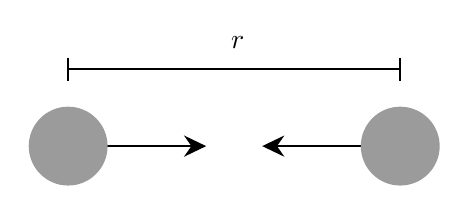
\begin{tikzpicture}[x=0.75pt,y=0.75pt,yscale=-1,xscale=1]
		%uncomment if require: \path (0,300); %set diagram left start at 0, and has height of 300

		%Straight Lines [id:da8632282549610462] 
		\draw    (141.25,180.75) -- (204.75,180.75) ;
		\draw [shift={(207.75,180.75)}, rotate = 180] [fill={rgb, 255:red, 0; green, 0; blue, 0 }  ][line width=0.08]  [draw opacity=0] (10.72,-5.15) -- (0,0) -- (10.72,5.15) -- (7.12,0) -- cycle    ;
		%Shape: Circle [id:dp9617032101256509] 
		\draw  [draw opacity=0][fill={rgb, 255:red, 155; green, 155; blue, 155 }  ,fill opacity=1 ] (122.25,180.75) .. controls (122.25,170.26) and (130.76,161.75) .. (141.25,161.75) .. controls (151.74,161.75) and (160.25,170.26) .. (160.25,180.75) .. controls (160.25,191.24) and (151.74,199.75) .. (141.25,199.75) .. controls (130.76,199.75) and (122.25,191.24) .. (122.25,180.75) -- cycle ;
		%Straight Lines [id:da06892075494490246] 
		\draw    (237.75,180.75) -- (301.25,180.75) ;
		\draw [shift={(234.75,180.75)}, rotate = 0] [fill={rgb, 255:red, 0; green, 0; blue, 0 }  ][line width=0.08]  [draw opacity=0] (10.72,-5.15) -- (0,0) -- (10.72,5.15) -- (7.12,0) -- cycle    ;
		%Shape: Circle [id:dp38068629635870566] 
		\draw  [draw opacity=0][fill={rgb, 255:red, 155; green, 155; blue, 155 }  ,fill opacity=1 ] (282.25,180.75) .. controls (282.25,170.26) and (290.76,161.75) .. (301.25,161.75) .. controls (311.74,161.75) and (320.25,170.26) .. (320.25,180.75) .. controls (320.25,191.24) and (311.74,199.75) .. (301.25,199.75) .. controls (290.76,199.75) and (282.25,191.24) .. (282.25,180.75) -- cycle ;
		%Straight Lines [id:da10419761541948369] 
		\draw    (141.25,143.75) -- (301.25,143.75) ;
		\draw [shift={(301.25,143.75)}, rotate = 180] [color={rgb, 255:red, 0; green, 0; blue, 0 }  ][line width=0.75]    (0,5.59) -- (0,-5.59)   ;
		\draw [shift={(141.25,143.75)}, rotate = 180] [color={rgb, 255:red, 0; green, 0; blue, 0 }  ][line width=0.75]    (0,5.59) -- (0,-5.59)   ;

		% Text Node
		\draw (223,131) node    {$r$};

		\end{tikzpicture}
	\end{figure}
	
	Dove il segno meno sta ad indicare che la forza è attrattiva.
	\item Interazione elettromagnetica: è una forza molto simile alla precedente ma che dipende dalla carica dei corpi. In particolare corpi carichi con lo stesso segno si respingono, corpi carichi con diverso segno si attraggono. È una forza che nel tempo dà luogo alle onde elettromagnetiche e per questo è estremamente importante.
	\item Interazione nucleare forte. Quando due corpi dotati della stessa carica sono vicini si respingono.  Questa forza permette di mantenere la stabilità del nucleo, attrae i protoni fra di loro in modo tale che l'atomo rimanga compatto e ha un raggio di interazione estremamente corto. Quindi fuori dai nuclei praticamente è inesistente.
	\item Interazione nucleare debole: interazione fra gli elettroni che permette di spiegare l'esistenza dei decadimenti radioattivi, quando un atomo instabile emette una radiazione e diventa un altro elemento.
\end{itemize}

Tutte le altre forze sono casi particolari che rientrano in queste categorie. La scoperta che l'apparente grande varietà di tipi di forze è il manifestarsi di poche interazioni fondamentali, assume una grande rilevanza concettuale ed è il risultato di una lunga indagine sperimentale e teorica rivolta all'unificazione delle interazioni.

\subsection{Esempi di forze}

Le forze possono essere classificate in attive e reattive (o vincolari).

\subsubsection{Forze attive}

Si tratta di quelle forze che non sono dovute a un vincolo.

\paragraph{Forza peso} Avendo introdotto l'interazione gravitazionale, è possibile capire perché tutti i corpi sulla superficie terrestre sono accelerati verso il centro della Terra. Essi infatti risentono dell'attrazione di quest'ultima che ha una massa molto grande. Questa forza attrattiva prende il nome di forza peso. Essa si considera costante in modulo per tutti i corpi prossimi alla superficie terrestre perché la loro distanza da essa è molto piccola in confronto al suo raggio. Viene definita una costante $g$ che prende il nome di accelerazione di gravità perché il suo prodotto per la massa da una forza. Si trova che $g=9.81 \frac{m}{s^2}$. Tutti i corpi sono accelerati verso il centro della Terra con intensità proporzionale alla propria massa. Per trasformarla in una relazione vettoriale si definisce $\vec{g}$ come un vettore che punta sempre verso il centro della Terra e che quindi permette di dire che la forza peso vale, per la seconda legge della dinamica:

\[
	\vec{F}_{peso}=m\vec{g}
\]

Un corpo che cade nell'aria in realtà presenta un'accelerazione minore di quella di gravità a causa dell'attrito con l'aria. La proporzionalità fra peso e massa suggerisce che il confronto tra due masse possa essere effettuato confrontando le rispettive forze peso. Tale fatto non deve però portare a confondere i due concetti di massa e forza peso. La prima ha significato dinamico indipendente dalla forza agente, mentre la seconda risulta dall'interazione di un corpo con la Terra. Sulla superficie di un altro pianeta essa sarebbe diversa a causa del diverso valore di $g$.

\paragraph{Forza elettrica} Dati due corpi dotati di carica $q_1$ e $q_2$ si esercita una forza fra di essi inversamente proporzionale al quadrato della loro distanza e proporzionale al prodotto delle loro cariche secondo una costante di proporzionalità $k$. La si esprime tramite il versore radiale. Se i due corpi sono dotati della stessa carica, la forza diventa equiversa a $\vec{u}_r$. Essa è responsabile di molti fenomeni osservati in natura.

\paragraph{Forza elastica} Quando un corpo è in grado di allungarsi, nasce una forza di richiamo che prende il nome di \emph{forza elastica}, la quale vorrebbe riportare il corpo nella sua posizione di riposo. Si può dimostrare che questa forza elastica è direttamente proporzionale all'allungamento $\vec{\Delta L}$ tramite una costante di proporzionalità detta costante elastica della molla.

\[
	\vec{F}=-k\vec{\Delta L}
\]

Il segno meno nasce perché la forza agisce in direzione parallela all'allungamento ma con verso opposto ad esso per richiamare il corpo indietro. Il segno invece non va cambiato se la molla viene accorciata.

\begin{figure}[htpb]
	\centering

	\tikzset{every picture/.style={line width=0.75pt}} %set default line width to 0.75pt        

	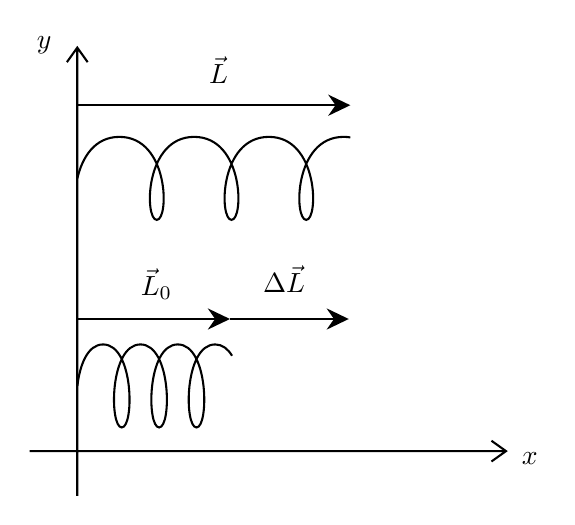
\begin{tikzpicture}[x=0.75pt,y=0.75pt,yscale=-1,xscale=1]
	%uncomment if require: \path (0,300); %set diagram left start at 0, and has height of 300

	%Shape: Axis 2D [id:dp001535704915357261] 
	\draw  (106,245.4) -- (335.5,245.4)(128.95,51) -- (128.95,267) (328.5,240.4) -- (335.5,245.4) -- (328.5,250.4) (123.95,58) -- (128.95,51) -- (133.95,58)  ;
	%Shape: Spring [id:dp05311315184863874] 
	\draw   (129,114) .. controls (131.25,104) and (137.25,94) .. (149.25,94) .. controls (173.25,94) and (173.25,134) .. (167.25,134) .. controls (161.25,134) and (161.25,94) .. (185.25,94) .. controls (209.25,94) and (209.25,134) .. (203.25,134) .. controls (197.25,134) and (197.25,94) .. (221.25,94) .. controls (245.25,94) and (245.25,134) .. (239.25,134) .. controls (233.25,134) and (233.25,94) .. (257.25,94) .. controls (258.39,94) and (259.47,94.09) .. (260.5,94.26) ;
	%Shape: Spring [id:dp7319432525707565] 
	\draw   (129,214) .. controls (130.13,204) and (133.88,194) .. (141.38,194) .. controls (156.38,194) and (156.38,234) .. (150.38,234) .. controls (144.38,234) and (144.38,194) .. (159.38,194) .. controls (174.38,194) and (174.38,234) .. (168.38,234) .. controls (162.38,234) and (162.38,194) .. (177.38,194) .. controls (192.38,194) and (192.38,234) .. (186.38,234) .. controls (180.38,234) and (180.38,194) .. (195.38,194) .. controls (198.85,194) and (201.52,196.15) .. (203.5,199.45) ;
	%Straight Lines [id:da6026322365253902] 
	\draw    (129.25,78.75) -- (257.5,78.75) ;
	\draw [shift={(260.5,78.75)}, rotate = 180] [fill={rgb, 255:red, 0; green, 0; blue, 0 }  ][line width=0.08]  [draw opacity=0] (10.72,-5.15) -- (0,0) -- (10.72,5.15) -- (7.12,0) -- cycle    ;
	%Straight Lines [id:da9991989473762817] 
	\draw    (129.25,181.75) -- (199.5,181.75) ;
	\draw [shift={(202.5,181.75)}, rotate = 180] [fill={rgb, 255:red, 0; green, 0; blue, 0 }  ][line width=0.08]  [draw opacity=0] (10.72,-5.15) -- (0,0) -- (10.72,5.15) -- (7.12,0) -- cycle    ;
	%Straight Lines [id:da5075934876195309] 
	\draw    (202.5,181.75) -- (256.75,181.75) ;
	\draw [shift={(259.75,181.75)}, rotate = 180] [fill={rgb, 255:red, 0; green, 0; blue, 0 }  ][line width=0.08]  [draw opacity=0] (10.72,-5.15) -- (0,0) -- (10.72,5.15) -- (7.12,0) -- cycle    ;

	% Text Node
	\draw (347,249) node    {$x$};
	% Text Node
	\draw (113,50) node    {$y$};
	% Text Node
	\draw (197,62) node    {$\vec{L}$};
	% Text Node
	\draw (167.06,165) node    {$\vec{L}_{0}$};
	% Text Node
	\draw (228.6,162.6) node    {$\Delta \vec{L}$};

	\end{tikzpicture}
\end{figure}

Si consideri una molla: quando $k$ è alta vuole dire che a pari allungamento essa genererà una forza di richiamo notevole (e che si dovrà applicare una forza notevole per deformarla). In questo caso si parla di \textbf{molla rigida}. Le molle che si deformano facilmente prendono invece il nome di \textbf{molle lasche}.

\paragraph{Tensione dei fili} Tra le forze attive figura anche la tensione, interazione che si manifesta quando si collegano i corpi con funi, che verranno considerate prive di estensione. Una fune è un oggetto che per definizione può sopportare solo forze di trazione; se viene compressa si deforma. La tensione si ha quando la fune è tesa ed è una forza diretta parallelamente alla direzione della fune stessa. In genere viene indicata con $\vec{T}$.  Si considererà in seguito una fune:

\begin{itemize}
	\item di massa trascurabile, approssimabile a $0$. Questa idealizzazione ha un'importante conseguenza:
	\[
		\vec{T}_b-\vec{T}_a=m_{\text{fune}}\,\vec{a}=0 \implies \vec{T}_b=\vec{T}_a
	\]
	Significa che in ogni punto la fune è soggetta alla stessa tensione.
	\item inestensibile, non elastica. Ciò significa che mantiene lunghezza costante e che quindi tutti i suoi punti si muovono con stessa velocità e stessa accelerazione in ogni istante di tempo. Per questo la fune è utile per collegare due corpi e farli muovere alla stessa velocità.
\end{itemize}

\begin{figure}[htpb]
	\centering

	\tikzset{every picture/.style={line width=0.75pt}} %set default line width to 0.75pt        

	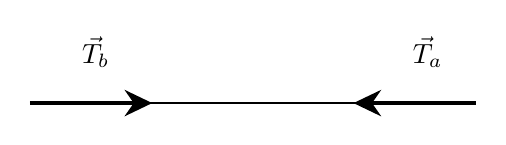
\begin{tikzpicture}[x=0.75pt,y=0.75pt,yscale=-1,xscale=1]
	%uncomment if require: \path (0,300); %set diagram left start at 0, and has height of 300

	%Straight Lines [id:da4135641760741906] 
	\draw    (198.5,139) -- (413.5,139) ;
	%Straight Lines [id:da41024725268239504] 
	\draw [line width=1.5]    (198.5,139) -- (253.5,139) ;
	\draw [shift={(257.5,139)}, rotate = 180] [fill={rgb, 255:red, 0; green, 0; blue, 0 }  ][line width=0.08]  [draw opacity=0] (13.4,-6.43) -- (0,0) -- (13.4,6.44) -- (8.9,0) -- cycle    ;
	%Straight Lines [id:da6068473195480548] 
	\draw [line width=1.5]    (358.5,139) -- (413.5,139) ;
	\draw [shift={(354.5,139)}, rotate = 0] [fill={rgb, 255:red, 0; green, 0; blue, 0 }  ][line width=0.08]  [draw opacity=0] (13.4,-6.43) -- (0,0) -- (13.4,6.44) -- (8.9,0) -- cycle    ;

	% Text Node
	\draw (230.27,114.56) node    {$\vec{T}_{b}$};
	% Text Node
	\draw (390.27,114.56) node    {$\vec{T}_{a}$};

	\end{tikzpicture}
\end{figure}

Riassumendo, il filo teso esercita agli estremi la tensione $\vec{T}$, il cui valore dipende dalle forze applicate, e che deve essere pensata come la reazione del filo alla forza che lo tende. Per un filo reale la tensione non può superare un valore massimo oltre al quale esso si spezza. Questo valore dipende dalla sostanza con cui è fatto il filo e dalle sue dimensioni geometriche.

Si consideri due corpi collegati ad un filo. Per quanto appena detto, essi presentano la stessa accelerazione. $m_2$ risente anche di una forza esercitata da $m_1$ pari a $\vec{T}$.

\begin{figure}[htpb]
	\centering

	\tikzset{every picture/.style={line width=0.75pt}} %set default line width to 0.75pt        

	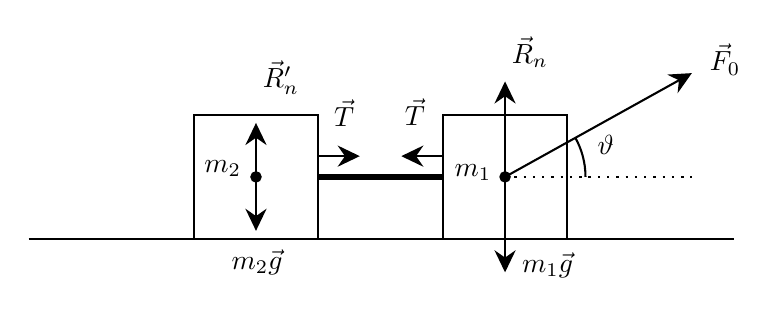
\begin{tikzpicture}[x=0.75pt,y=0.75pt,yscale=-1,xscale=1]
	%uncomment if require: \path (0,300); %set diagram left start at 0, and has height of 300

	%Shape: Rectangle [id:dp13182710929166452] 
	\draw   (190,110) -- (250,110) -- (250,170) -- (190,170) -- cycle ;
	%Shape: Rectangle [id:dp8276676004174683] 
	\draw   (310,110) -- (370,110) -- (370,170) -- (310,170) -- cycle ;
	%Straight Lines [id:da34170094100934567] 
	\draw [line width=2.25]    (250,140) -- (310,140) ;
	%Straight Lines [id:da48469720672133] 
	\draw [line width=0.75]    (250,130) -- (267,130) ;
	\draw [shift={(270,130)}, rotate = 180] [fill={rgb, 255:red, 0; green, 0; blue, 0 }  ][line width=0.08]  [draw opacity=0] (10.72,-5.15) -- (0,0) -- (10.72,5.15) -- (7.12,0) -- cycle    ;
	%Straight Lines [id:da6470155408923426] 
	\draw [line width=0.75]    (310,130) -- (293,130) ;
	\draw [shift={(290,130)}, rotate = 360] [fill={rgb, 255:red, 0; green, 0; blue, 0 }  ][line width=0.08]  [draw opacity=0] (10.72,-5.15) -- (0,0) -- (10.72,5.15) -- (7.12,0) -- cycle    ;
	%Straight Lines [id:da6637094186690098] 
	\draw [line width=0.75]    (340,140) -- (340,183) ;
	\draw [shift={(340,186)}, rotate = 270] [fill={rgb, 255:red, 0; green, 0; blue, 0 }  ][line width=0.08]  [draw opacity=0] (10.72,-5.15) -- (0,0) -- (10.72,5.15) -- (7.12,0) -- cycle    ;
	%Straight Lines [id:da8958397597628005] 
	\draw [line width=0.75]  [dash pattern={on 0.84pt off 2.51pt}]  (340,140) -- (430,140) ;
	%Straight Lines [id:da2860240635593594] 
	\draw [line width=0.75]    (340,140) -- (427.38,91.46) ;
	\draw [shift={(430,90)}, rotate = 510.95] [fill={rgb, 255:red, 0; green, 0; blue, 0 }  ][line width=0.08]  [draw opacity=0] (10.72,-5.15) -- (0,0) -- (10.72,5.15) -- (7.12,0) -- cycle    ;
	%Straight Lines [id:da12525197401114996] 
	\draw [line width=0.75]    (340,97) -- (340,140) ;
	\draw [shift={(340,94)}, rotate = 90] [fill={rgb, 255:red, 0; green, 0; blue, 0 }  ][line width=0.08]  [draw opacity=0] (10.72,-5.15) -- (0,0) -- (10.72,5.15) -- (7.12,0) -- cycle    ;
	%Straight Lines [id:da264838336587333] 
	\draw [line width=0.75]    (220,117) -- (220,140) ;
	\draw [shift={(220,114)}, rotate = 90] [fill={rgb, 255:red, 0; green, 0; blue, 0 }  ][line width=0.08]  [draw opacity=0] (10.72,-5.15) -- (0,0) -- (10.72,5.15) -- (7.12,0) -- cycle    ;
	%Straight Lines [id:da24672318102456936] 
	\draw [line width=0.75]    (220,140) -- (220,163) ;
	\draw [shift={(220,166)}, rotate = 270] [fill={rgb, 255:red, 0; green, 0; blue, 0 }  ][line width=0.08]  [draw opacity=0] (10.72,-5.15) -- (0,0) -- (10.72,5.15) -- (7.12,0) -- cycle    ;
	%Shape: Circle [id:dp3108503584894222] 
	\draw  [fill={rgb, 255:red, 0; green, 0; blue, 0 }  ,fill opacity=1 ] (217.75,140) .. controls (217.75,138.76) and (218.76,137.75) .. (220,137.75) .. controls (221.24,137.75) and (222.25,138.76) .. (222.25,140) .. controls (222.25,141.24) and (221.24,142.25) .. (220,142.25) .. controls (218.76,142.25) and (217.75,141.24) .. (217.75,140) -- cycle ;
	%Shape: Circle [id:dp06572143906472427] 
	\draw  [fill={rgb, 255:red, 0; green, 0; blue, 0 }  ,fill opacity=1 ] (337.75,140) .. controls (337.75,138.76) and (338.76,137.75) .. (340,137.75) .. controls (341.24,137.75) and (342.25,138.76) .. (342.25,140) .. controls (342.25,141.24) and (341.24,142.25) .. (340,142.25) .. controls (338.76,142.25) and (337.75,141.24) .. (337.75,140) -- cycle ;
	%Shape: Arc [id:dp8957298166828258] 
	\draw  [draw opacity=0] (373.8,121.04) .. controls (376.95,126.64) and (378.75,133.11) .. (378.75,140) -- (340,140) -- cycle ; \draw   (373.8,121.04) .. controls (376.95,126.64) and (378.75,133.11) .. (378.75,140) ;
	%Straight Lines [id:da6733190100538535] 
	\draw [line width=0.75]    (110.5,170) -- (450.5,170) ;

	% Text Node
	\draw (204,136) node    {$m_{2}$};
	% Text Node
	\draw (324.5,138) node    {$m_{1}$};
	% Text Node
	\draw (262.5,109.5) node    {$\vec{T}$};
	% Text Node
	\draw (296.5,109) node    {$\vec{T}$};
	% Text Node
	\draw (352,80) node    {$\vec{R}_{n}$};
	% Text Node
	\draw (232,92) node    {$\vec{R} '_{n}$};
	% Text Node
	\draw (220.5,181) node    {$m_{2}\vec{g}$};
	% Text Node
	\draw (360.5,182.5) node    {$m_{1}\vec{g}$};
	% Text Node
	\draw (446,83.5) node    {$\vec{F}_{0}$};
	% Text Node
	\draw (388.5,124.5) node    {$\vartheta $};

	\end{tikzpicture}
\end{figure}

\begin{gather*}
	F_0\cos\vartheta=(m_1+m_2)\,a \\
	R_n=m_2 g-F_0\sin\vartheta \quad \text{condizione essenziale è che} \quad F_0\sin\vartheta<m_2 g,
\end{gather*}

altrimenti il corpo verrebbe sollevato e non si avrebbe più contatto.

\subsubsection{Reazioni vincolari}

Gli oggetti possono anche interagire essendo soggetti a vincoli: quando il punto materiale è posto ad esempio su un piano, questo impone dei vincoli alla sua posizione. Infatti, se un corpo soggetto all'azione di una forza o della risultante non nulla di un insieme di forze, rimane fermo, bisogna dedurre l'esistenza di una reazione dell'ambiente circostante, detta \textbf{reazione vincolare}, applicata al corpo stesso in modo che rimanga in quiete. I vincoli fanno si che l'oggetto non possa occupare tutte le posizioni possibili nello spazio. Le reazioni vincolari sono quindi forze esercitate dal vincolo sul corpo e con verso sempre opposto al tentativo di spostamento del corpo. Si affrontano in seguito alcuni esempi di reazioni vincolari.

\paragraph{Reazioni normali} Tutte le volte che c'è un vincolo esiste sempre una forza generata da esso al corpo diretta perpendicolarmente al piano d'appoggio: \textbf{reazione normale}. Ad esempio, l'oggetto sarà sempre accelerato verso il centro della Terra, sarà soggetto alla forza peso, ma non sfonderà il piano d'appoggio perché questo si sta comportando da vincolo ed esercita su di esso una forza diretta da se verso l'esterno, ortogonale al piano.

\[
	m\vec{g}-\vec{R}_n=0
\]

\begin{figure}[htpb]
	\centering

	\tikzset{every picture/.style={line width=0.75pt}} %set default line width to 0.75pt        

	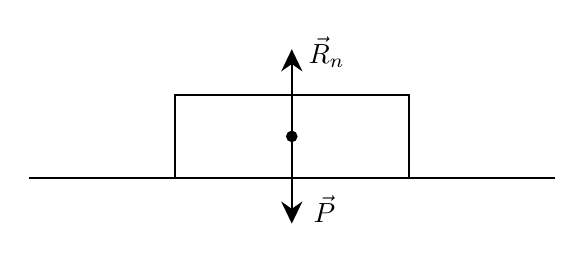
\begin{tikzpicture}[x=0.75pt,y=0.75pt,yscale=-1,xscale=1]
	%uncomment if require: \path (0,300); %set diagram left start at 0, and has height of 300

	%Shape: Rectangle [id:dp5690079782842519] 
	\draw   (170.5,118) -- (283,118) -- (283,158) -- (170.5,158) -- cycle ;
	%Straight Lines [id:da7512390417384545] 
	\draw    (100,158) -- (353.5,158) ;
	%Straight Lines [id:da45126245871489656] 
	\draw    (226.75,138) -- (226.75,177) ;
	\draw [shift={(226.75,180)}, rotate = 270] [fill={rgb, 255:red, 0; green, 0; blue, 0 }  ][line width=0.08]  [draw opacity=0] (10.72,-5.15) -- (0,0) -- (10.72,5.15) -- (7.12,0) -- cycle    ;
	%Straight Lines [id:da9581308585695909] 
	\draw    (226.75,99) -- (226.75,138) ;
	\draw [shift={(226.75,96)}, rotate = 90] [fill={rgb, 255:red, 0; green, 0; blue, 0 }  ][line width=0.08]  [draw opacity=0] (10.72,-5.15) -- (0,0) -- (10.72,5.15) -- (7.12,0) -- cycle    ;
	%Shape: Circle [id:dp39805459767111984] 
	\draw  [fill={rgb, 255:red, 0; green, 0; blue, 0 }  ,fill opacity=1 ] (224.5,138) .. controls (224.5,136.76) and (225.51,135.75) .. (226.75,135.75) .. controls (227.99,135.75) and (229,136.76) .. (229,138) .. controls (229,139.24) and (227.99,140.25) .. (226.75,140.25) .. controls (225.51,140.25) and (224.5,139.24) .. (224.5,138) -- cycle ;

	% Text Node
	\draw (243.5,97.5) node    {$\vec{R}_n$};
	% Text Node
	\draw (242.5,173) node    {$\vec{P}$};

	\end{tikzpicture}
\end{figure}
\FloatBarrier
Ovviamente esisterà un valore massimo della reazione normale che può essere esercitata dal piano d'appoggio, detto \textbf{carico di rottura}, al di sotto del quale si mantiene $\vec{R}_n$. Si potrebbe pensare che questa reazione normale rappresenti una coppia di forze responsabili del principio azione reazione, ma ciò non può essere vero perché le due forze sono applicate allo stesso corpo.

\subparagraph{Piano inclinato} Si consideri un corpo, assimilabile ad un punto materiale di massa $m$, che possa muoversi sotto l'azione del suo peso, su una superficie piana inclinata di un angolo $\vartheta$ rispetto al piano orizzontale. L'obbiettivo è quello di ricavare la legge oraria del moto. Il corpo sarà sicuramente soggetto all'accelerazione di gravità, ma il vincolo a cui è appoggiato fa si che non cada: esiste sempre una reazione normale generata dal piano d'appoggio. Si supponga che non ci sia attrito. Note queste forze si scrive la seconda legge della dinamica per ricavare la legge oraria. L'oggetto si muove lungo il piano inclinato quindi conviene definire come sistema di riferimento un asse parallelo e uno perpendicolare al piano.

\begin{figure}[htpb]
	\centering

	\tikzset{every picture/.style={line width=0.75pt}} %set default line width to 0.75pt        

	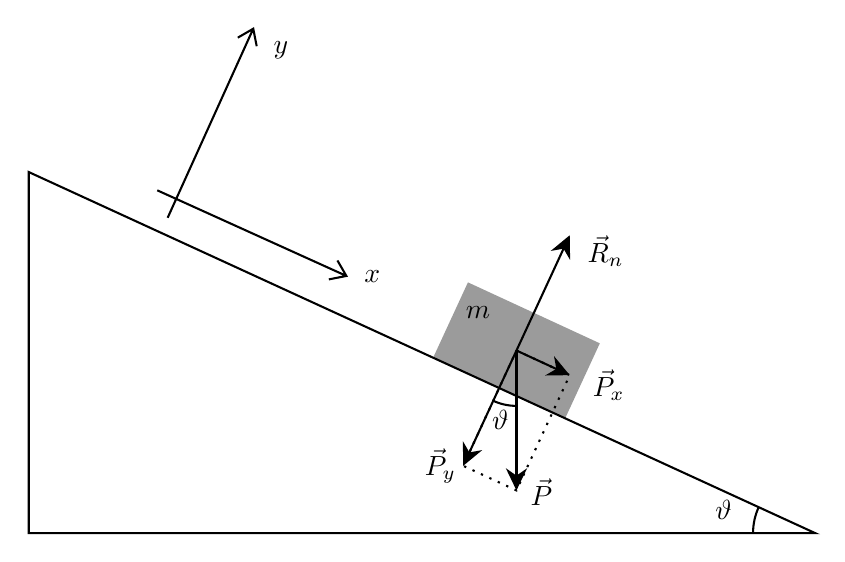
\begin{tikzpicture}[x=0.75pt,y=0.75pt,yscale=-1,xscale=1]
	%uncomment if require: \path (0,300); %set diagram left start at 0, and has height of 300

	%Shape: Rectangle [id:dp6463061738178288] 
	\draw  [draw opacity=0][fill={rgb, 255:red, 155; green, 155; blue, 155 }  ,fill opacity=1 ] (311.62,133.16) -- (375.16,162.53) -- (358.38,198.84) -- (294.84,169.47) -- cycle ;
	%Shape: Right Triangle [id:dp6144937690601591] 
	\draw   (100,80) -- (478.98,254) -- (100,254) -- cycle ;
	%Shape: Axis 2D [id:dp5829870105582096] 
	\draw  (161.95,88.82) -- (253.05,130.06)(208.18,10.95) -- (166.94,102.05) (248.74,122.62) -- (253.05,130.06) -- (244.61,131.73) (200.74,15.27) -- (208.18,10.95) -- (209.85,19.39)  ;
	%Straight Lines [id:da9706510721340091] 
	\draw    (335,166) -- (335,230.4) ;
	\draw [shift={(335,233.4)}, rotate = 270] [fill={rgb, 255:red, 0; green, 0; blue, 0 }  ][line width=0.08]  [draw opacity=0] (10.72,-5.15) -- (0,0) -- (10.72,5.15) -- (7.12,0) -- cycle    ;
	%Straight Lines [id:da5886444887800437] 
	\draw    (335,166) -- (310.59,218.82) ;
	\draw [shift={(309.34,221.54)}, rotate = 294.8] [fill={rgb, 255:red, 0; green, 0; blue, 0 }  ][line width=0.08]  [draw opacity=0] (10.72,-5.15) -- (0,0) -- (10.72,5.15) -- (7.12,0) -- cycle    ;
	%Straight Lines [id:da8594044013143456] 
	\draw    (335,166) -- (357.94,176.6) ;
	\draw [shift={(360.66,177.86)}, rotate = 204.8] [fill={rgb, 255:red, 0; green, 0; blue, 0 }  ][line width=0.08]  [draw opacity=0] (10.72,-5.15) -- (0,0) -- (10.72,5.15) -- (7.12,0) -- cycle    ;
	%Straight Lines [id:da05616414654235857] 
	\draw    (359.41,113.18) -- (335,166) ;
	\draw [shift={(360.66,110.46)}, rotate = 114.8] [fill={rgb, 255:red, 0; green, 0; blue, 0 }  ][line width=0.08]  [draw opacity=0] (10.72,-5.15) -- (0,0) -- (10.72,5.15) -- (7.12,0) -- cycle    ;
	%Shape: Arc [id:dp2348034454786576] 
	\draw  [draw opacity=0] (335.06,192.67) .. controls (335.04,192.67) and (335.02,192.67) .. (335,192.67) .. controls (330.94,192.67) and (327.1,191.76) .. (323.66,190.14) -- (335,166) -- cycle ; \draw   (335.06,192.67) .. controls (335.04,192.67) and (335.02,192.67) .. (335,192.67) .. controls (330.94,192.67) and (327.1,191.76) .. (323.66,190.14) ;
	%Shape: Arc [id:dp3867135949818161] 
	\draw  [draw opacity=0] (448.98,253.85) .. controls (449,249.36) and (450.01,245.11) .. (451.79,241.29) -- (478.98,254) -- cycle ; \draw   (448.98,253.85) .. controls (449,249.36) and (450.01,245.11) .. (451.79,241.29) ;
	%Shape: Rectangle [id:dp07831331870274494] 
	\draw  [dash pattern={on 0.84pt off 2.51pt}] (335,166) -- (360.66,177.86) -- (335,233.4) -- (309.34,221.54) -- cycle ;

	% Text Node
	\draw (221.5,21.5) node    {$y$};
	% Text Node
	\draw (378,118) node    {$\vec{R}_{n}$};
	% Text Node
	\draw (379.5,182.67) node    {$\vec{P}_{x}$};
	% Text Node
	\draw (298.33,221.67) node    {$\vec{P}_{y}$};
	% Text Node
	\draw (434.83,243) node    {$\vartheta $};
	% Text Node
	\draw (265.5,130.5) node    {$x$};
	% Text Node
	\draw (327.17,199.33) node    {$\vartheta $};
	% Text Node
	\draw (347,234) node    {$\vec{P}$};
	% Text Node
	\draw (316.5,147.67) node    {$m$};

	\end{tikzpicture}
\end{figure}

\begin{align*}
	x&: \quad P_x=P\sin\vartheta=mg\sin\vartheta \quad a=g\sin\vartheta=\text{costante} \\
	y&: \quad P_y-R_n=mgsin\vartheta-R_n=0 \quad (\text{non c'è moto sull'asse $y$})
\end{align*}

Si noti che si ha $a=g\sin\vartheta$: il corpo scende con moto uniformemente accelerato (infatti $a$ non dipende dal tempo) e l'accelerazione è minore di quella di gravità.

\[
	\vec{F}=m\vec{a} \implies \begin{cases} mg\sin\vartheta=ma \\ mg\cos\vartheta=R_n \end{cases}
\]

\paragraph{Forza d'attrito} Quanto visto in precedenza è valido se i vincoli sono perfettamente lisci. Se invece ciò non accade, la reazione normale continua ad esistere ma oltre ad essa agisce anche un altra reazione vincolare, questa volta tangente al vincolo, che prende il nome di \textbf{forza di attrito}. Ci sono diverse forme di attrito a seconda delle situazioni e dei fenomeni fisici che si possono considerare:

\begin{itemize}
	\item attrito \emph{radente}: generato dallo strisciamento di un corpo su una superficie senza rotolamento;
	\item attrito \emph{volvente}: che si manifesta in presenza di rotolamento e traslazione;
	\item attrito \emph{viscoso}: generato dal moto di un corpo in un fluido.
\end{itemize}

Si comincia studiando la forza di attrito radente. Ne esistono due tipologie:

\begin{itemize}
	\item statico. Si oppone al tentativo di movimento e permette a un corpo soggetto a forze di rimanere in equilibrio. A livello microscopico accade che tra i due corpi, le cariche presenti sulla superficie si attraggono e le zone rugose, grazie all'attrazione elettrostatica, vanno a creare delle microfusioni sulla superficie di contatto. Se il corpo non si muove significa che non si sono spezzate queste microfusioni. Si può dimostrare che la forza di attrito radente statico può assumere tutti valori possibili al di sotto di un valore che corrisponde alla situazione in cui si vanno a rompere le microfusioni che si formano. Questo valore massimo, nel caso dell'attrito statico, non dipende dall'estensione della superficie di contatto ma da quanto sono rugosi i due corpi interessati, aspetto che si caratterizza con il \emph{coefficiente di attrito statico} $\mu_s$, e da quanto il corpo sta scaricando sul piano il suo peso.
	\begin{gather*}
		\vec{R}_{t, max}=-\mu_s\,\norm{\vec{R}_n}\,\vec{u}_t \\
		\norm{\vec{F}_0}<\norm{\vec{R}_{t, max}} \implies \text{il corpo è fermo}
	\end{gather*}
	\item dinamico. Si ha quando si applica una forza maggiore di $\vec{R}_{t, max}$ e il corpo di conseguenza si muove. Anche in questo caso $\vec{R}(t)$ non è un valore noto a priori. In condizioni dinamiche il modulo di $\vec{R}(t)$ è pari a:
	\[
		\norm{\vec{R}_t}=\mu_d\,\norm{\vec{R}_{n}}
	\]
	Dove $\mu_d$ è il coefficiente di attrito dinamico. Si può in generale affermare che il valore del coefficiente di attrito dinamico è inferiore a quello del coefficiente di attrito statico. Questo a indice del fatto che è più facile mantenere in movimento un corpo su un piano scabro che metterlo in moto. Infatti mentre il corpo si muove si continuano a rompere e formare le microfusioni.
\end{itemize}

\begin{figure}[htpb]
	\centering

	\tikzset{every picture/.style={line width=0.75pt}} %set default line width to 0.75pt        

	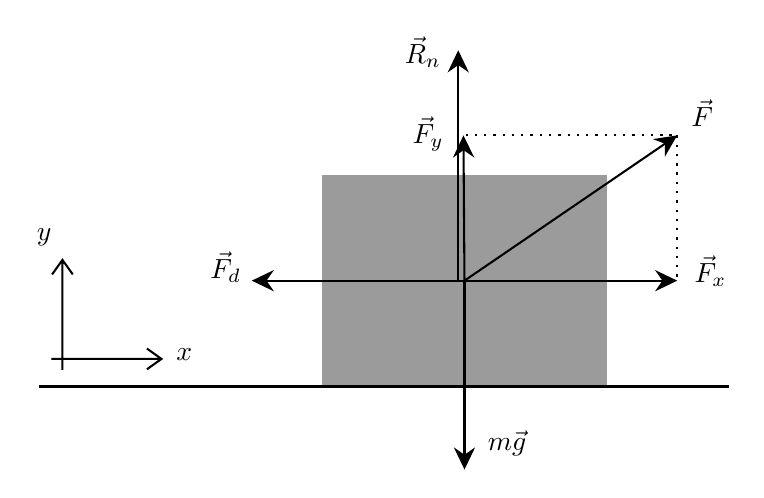
\begin{tikzpicture}[x=0.75pt,y=0.75pt,yscale=-1,xscale=1]
	%uncomment if require: \path (0,300); %set diagram left start at 0, and has height of 300

	%Shape: Rectangle [id:dp6376951996226576] 
	\draw  [draw opacity=0][fill={rgb, 255:red, 155; green, 155; blue, 155 }  ,fill opacity=1 ] (256.5,88) -- (393.5,88) -- (393.5,190) -- (256.5,190) -- cycle ;
	%Straight Lines [id:da8345620016239454] 
	\draw    (322,31) -- (322,139) ;
	\draw [shift={(322,28)}, rotate = 90] [fill={rgb, 255:red, 0; green, 0; blue, 0 }  ][line width=0.08]  [draw opacity=0] (10.72,-5.15) -- (0,0) -- (10.72,5.15) -- (7.12,0) -- cycle    ;
	%Shape: Axis 2D [id:dp5030880839594016] 
	\draw  (126,176.7) -- (179,176.7)(131.3,129) -- (131.3,182) (172,171.7) -- (179,176.7) -- (172,181.7) (126.3,136) -- (131.3,129) -- (136.3,136)  ;
	%Straight Lines [id:da0665208633718779] 
	\draw    (120,190) -- (452.5,190) ;
	%Straight Lines [id:da5325951964673605] 
	\draw    (325,139) -- (325,227) ;
	\draw [shift={(325,230)}, rotate = 270] [fill={rgb, 255:red, 0; green, 0; blue, 0 }  ][line width=0.08]  [draw opacity=0] (10.72,-5.15) -- (0,0) -- (10.72,5.15) -- (7.12,0) -- cycle    ;
	%Straight Lines [id:da2420420382705757] 
	\draw    (325,139) -- (424.5,139) ;
	\draw [shift={(427.5,139)}, rotate = 180] [fill={rgb, 255:red, 0; green, 0; blue, 0 }  ][line width=0.08]  [draw opacity=0] (10.72,-5.15) -- (0,0) -- (10.72,5.15) -- (7.12,0) -- cycle    ;
	%Straight Lines [id:da8646744635567805] 
	\draw    (225.5,139) -- (325,139) ;
	\draw [shift={(222.5,139)}, rotate = 0] [fill={rgb, 255:red, 0; green, 0; blue, 0 }  ][line width=0.08]  [draw opacity=0] (10.72,-5.15) -- (0,0) -- (10.72,5.15) -- (7.12,0) -- cycle    ;
	%Straight Lines [id:da6574678032655001] 
	\draw    (325,139) -- (425.02,70.69) ;
	\draw [shift={(427.5,69)}, rotate = 505.67] [fill={rgb, 255:red, 0; green, 0; blue, 0 }  ][line width=0.08]  [draw opacity=0] (10.72,-5.15) -- (0,0) -- (10.72,5.15) -- (7.12,0) -- cycle    ;
	%Straight Lines [id:da317383377325658] 
	\draw    (325,139) -- (324.52,72) ;
	\draw [shift={(324.5,69)}, rotate = 449.59] [fill={rgb, 255:red, 0; green, 0; blue, 0 }  ][line width=0.08]  [draw opacity=0] (10.72,-5.15) -- (0,0) -- (10.72,5.15) -- (7.12,0) -- cycle    ;
	%Straight Lines [id:da8219185361646106] 
	\draw  [dash pattern={on 0.84pt off 2.51pt}]  (325.5,69) -- (427.5,69) ;
	%Straight Lines [id:da32767482553672544] 
	\draw  [dash pattern={on 0.84pt off 2.51pt}]  (427.5,69) -- (427.5,139) ;

	% Text Node
	\draw (305,29) node    {$\vec{R}_{n}$};
	% Text Node
	\draw (439.5,58.5) node    {$\vec{F}$};
	% Text Node
	\draw (443.5,134.5) node    {$\vec{F}_{x}$};
	% Text Node
	\draw (307.5,68.5) node    {$\vec{F}_{y}$};
	% Text Node
	\draw (210,132.5) node    {$\vec{F}_{d}$};
	% Text Node
	\draw (345.5,217.5) node    {$m\vec{g}$};
	% Text Node
	\draw (190,174.5) node    {$x$};
	% Text Node
	\draw (122.5,118) node    {$y$};

	\end{tikzpicture}
\end{figure}

Il coefficiente $\mu$ è un valore adimensionale perché lega una forza con una forza.

Come già anticipato, un corpo solido può muoversi anche in un fluido, sostanza gassosa o liquida. In questo tentativo di movimento, nasce una forza di reazione vincolare tangente al moto che prende il nome di \textbf{forza di attrito viscoso}.

\begin{figure}[htpb]
	\centering

	\tikzset{every picture/.style={line width=0.75pt}} %set default line width to 0.75pt        

	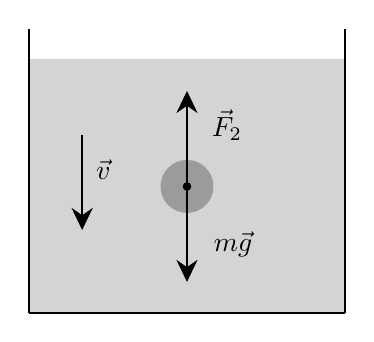
\begin{tikzpicture}[x=0.75pt,y=0.75pt,yscale=-1,xscale=1]
	%uncomment if require: \path (0,300); %set diagram left start at 0, and has height of 300

	%Shape: Rectangle [id:dp8561184232162118] 
	\draw  [draw opacity=0][fill={rgb, 255:red, 212; green, 212; blue, 212 }  ,fill opacity=1 ] (169,89.5) -- (321.5,89.5) -- (321.5,212) -- (169,212) -- cycle ;
	%Straight Lines [id:da7719242425976345] 
	\draw    (169,212) -- (321.5,212) ;
	%Straight Lines [id:da5058462018381182] 
	\draw    (169,212) -- (169,75) ;
	%Straight Lines [id:da6164225160919097] 
	\draw    (321.5,212) -- (321.5,75) ;
	%Shape: Circle [id:dp3166621773670002] 
	\draw  [draw opacity=0][fill={rgb, 255:red, 155; green, 155; blue, 155 }  ,fill opacity=1 ] (232.5,151) .. controls (232.5,143.96) and (238.21,138.25) .. (245.25,138.25) .. controls (252.29,138.25) and (258,143.96) .. (258,151) .. controls (258,158.04) and (252.29,163.75) .. (245.25,163.75) .. controls (238.21,163.75) and (232.5,158.04) .. (232.5,151) -- cycle ;
	%Straight Lines [id:da8089251880144308] 
	\draw    (245.25,151) -- (245.25,194) ;
	\draw [shift={(245.25,197)}, rotate = 270] [fill={rgb, 255:red, 0; green, 0; blue, 0 }  ][line width=0.08]  [draw opacity=0] (10.72,-5.15) -- (0,0) -- (10.72,5.15) -- (7.12,0) -- cycle    ;
	%Straight Lines [id:da7454704616065833] 
	\draw    (245.25,108) -- (245.25,151) ;
	\draw [shift={(245.25,105)}, rotate = 90] [fill={rgb, 255:red, 0; green, 0; blue, 0 }  ][line width=0.08]  [draw opacity=0] (10.72,-5.15) -- (0,0) -- (10.72,5.15) -- (7.12,0) -- cycle    ;
	%Shape: Circle [id:dp7293908222637295] 
	\draw  [draw opacity=0][fill={rgb, 255:red, 0; green, 0; blue, 0 }  ,fill opacity=1 ] (243.17,151) .. controls (243.17,149.85) and (244.1,148.92) .. (245.25,148.92) .. controls (246.4,148.92) and (247.33,149.85) .. (247.33,151) .. controls (247.33,152.15) and (246.4,153.08) .. (245.25,153.08) .. controls (244.1,153.08) and (243.17,152.15) .. (243.17,151) -- cycle ;
	%Straight Lines [id:da16874404501894302] 
	\draw    (194.75,126) -- (194.75,169) ;
	\draw [shift={(194.75,172)}, rotate = 270] [fill={rgb, 255:red, 0; green, 0; blue, 0 }  ][line width=0.08]  [draw opacity=0] (10.72,-5.15) -- (0,0) -- (10.72,5.15) -- (7.12,0) -- cycle    ;

	% Text Node
	\draw (264.5,121.5) node    {$\vec{F}_{2}$};
	% Text Node
	\draw (267.5,179) node    {$m\vec{g}$};
	% Text Node
	\draw (205,143) node    {$\vec{v}$};

	\end{tikzpicture}
\end{figure}
\FloatBarrier
Essa è proporzionale alla velocità del corpo soggetto a tale forza:

\[
	\vec{F}_{AV}=-\beta\vec{v} \implies \vec{a}=-\beta\frac{\vec{v}}{m}
\]
$\beta$ è il \emph{coefficiente di attrito viscoso} e dipende dalla forma del corpo, dalla sua velocità e dalla densità del fluido. Se la caduta del corpo avviene in un fluido non viscoso si avrà un moto rettilineo uniforme; altrimenti,  viene a nascere la forza di attrito viscoso che sottrae velocità; in particolar modo questa decresce in modo esponenziale nel tempo. Applicando infatti la legge di Newton,  posto $\beta=mk$ si ha:

\begin{gather*}
	\vec{F}_1+\vec{F}_2=m\vec{g}-mk\vec{v}=m\vec{a}=m\frac{d\vec{v}}{dt} \\
	\frac{dv}{dt}=g-kv \implies \frac{dv}{g-kv}=dt \implies t=\frac{\ln(g-kv)}{-k} \\
	\implies v(t)=\frac{g}{k}(1-e^{-kt})
\end{gather*}

Partendo da $0$ la velocità cresce, ma sempre più lentamente, per $t\gg\frac{1}{k}$, $v$ assume praticamente il valore costante $\frac{g}{k}$. In effetti si vede che per $v=\frac{g}{k}$ l'accelerazione diventa nulla. Questo risultato asintotico si ottiene anche considerando come varia con la velocità il modulo delle forze agenti: la forza peso è costante, mentre quella di attrito viscoso cresce linearmente con la velocità. Quando $v$ assume il valore $\frac{g}{k}$ si ha l'equilibrio dinamico tra le due forze e la loro risultante si annulla, di conseguenza si instaura un moto uniforme.

\begin{figure}[htpb]
	\centering

	\tikzset{every picture/.style={line width=0.75pt}} %set default line width to 0.75pt        

	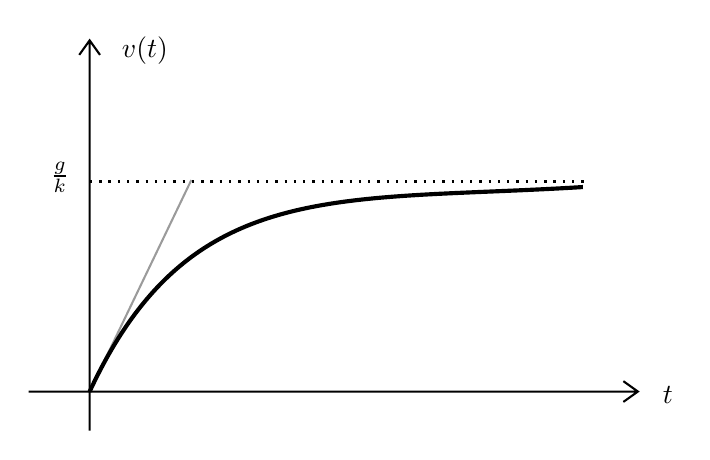
\begin{tikzpicture}[x=0.75pt,y=0.75pt,yscale=-1,xscale=1]
	%uncomment if require: \path (0,300); %set diagram left start at 0, and has height of 300

	%Straight Lines [id:da984137023687973] 
	\draw [color={rgb, 255:red, 155; green, 155; blue, 155 }  ,draw opacity=1 ]   (79.35,223.2) -- (128.33,121.33) ;
	%Shape: Axis 2D [id:dp5274226497252805] 
	\draw  (50,223.2) -- (343.5,223.2)(79.35,54) -- (79.35,242) (336.5,218.2) -- (343.5,223.2) -- (336.5,228.2) (74.35,61) -- (79.35,54) -- (84.35,61)  ;
	%Straight Lines [id:da9759819044033384] 
	\draw  [dash pattern={on 0.84pt off 2.51pt}]  (79.5,122) -- (320,122) ;
	% Plotting does not support converting to Tikz
	%Curve Lines [id:da034935606148249976] 
	\draw [line width=1.5]    (79.35,223.2) .. controls (127.67,119.33) and (198.33,132) .. (317,124.67) ;

	% Text Node
	\draw (106,59) node    {$v( t)$};
	% Text Node
	\draw (358,225) node    {$t$};
	% Text Node
	\draw (65,120) node    {$\frac{g}{k}$};

	\end{tikzpicture}
\end{figure}
\FloatBarrier

\subparagraph{Piano inclinato con attrito} Si riprenda il problema del corpo sul piano inclinato supponendo che esso sia scabro. Si immagini di poterne variare l'inclinazione a proprio piacimento. L'obbiettivo è di cercare l'angolo $\vartheta$ massimo al di sopra del quale il corpo si muove, mostrando che esso non dipende dalla massa del corpo.

\[
	\norm{\vec{P}_x} \le \norm{\vec{F}_d} = \norm{\vec{P}_y}\mu_s 	\implies mg\sin\vartheta\le mg\cos\vartheta \mu_s
\]

\begin{equation}
	\label{eqn:attrito}
	\tan\vartheta \le \mu_s
\end{equation}

\begin{figure}[htpb]
	\centering

	\tikzset{every picture/.style={line width=0.75pt}} %set default line width to 0.75pt        

	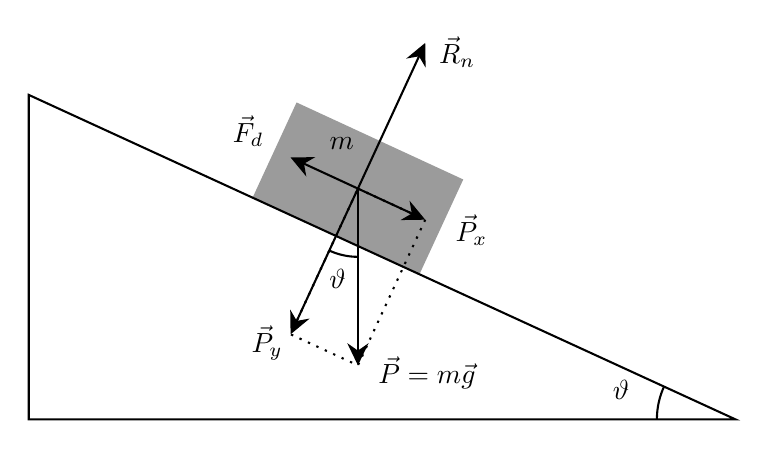
\begin{tikzpicture}[x=0.75pt,y=0.75pt,yscale=-1,xscale=1]
	%uncomment if require: \path (0,300); %set diagram left start at 0, and has height of 300

	%Shape: Rectangle [id:dp9393907316583523] 
	\draw  [draw opacity=0][fill={rgb, 255:red, 155; green, 155; blue, 155 }  ,fill opacity=1 ] (279.55,99.37) -- (359.86,136.48) -- (338.66,182.37) -- (258.35,145.26) -- cycle ;
	%Shape: Right Triangle [id:dp4374809228121763] 
	\draw   (150.5,95.72) -- (491.06,252.09) -- (150.5,252.09) -- cycle ;
	%Straight Lines [id:da23541904718549822] 
	\draw    (309.11,140.87) -- (309.11,223.05) ;
	\draw [shift={(309.11,226.05)}, rotate = 270] [fill={rgb, 255:red, 0; green, 0; blue, 0 }  ][line width=0.08]  [draw opacity=0] (10.72,-5.15) -- (0,0) -- (10.72,5.15) -- (7.12,0) -- cycle    ;
	%Straight Lines [id:da8160650307927853] 
	\draw    (309.11,140.87) -- (338.82,154.6) ;
	\draw [shift={(341.54,155.86)}, rotate = 204.8] [fill={rgb, 255:red, 0; green, 0; blue, 0 }  ][line width=0.08]  [draw opacity=0] (10.72,-5.15) -- (0,0) -- (10.72,5.15) -- (7.12,0) -- cycle    ;
	%Straight Lines [id:da4458617710302386] 
	\draw    (309.11,140.87) -- (277.93,208.34) ;
	\draw [shift={(276.67,211.07)}, rotate = 294.8] [fill={rgb, 255:red, 0; green, 0; blue, 0 }  ][line width=0.08]  [draw opacity=0] (10.72,-5.15) -- (0,0) -- (10.72,5.15) -- (7.12,0) -- cycle    ;
	%Straight Lines [id:da0008803172745237564] 
	\draw    (340.28,73.4) -- (309.11,140.87) ;
	\draw [shift={(341.54,70.68)}, rotate = 114.8] [fill={rgb, 255:red, 0; green, 0; blue, 0 }  ][line width=0.08]  [draw opacity=0] (10.72,-5.15) -- (0,0) -- (10.72,5.15) -- (7.12,0) -- cycle    ;
	%Shape: Arc [id:dp3140052717514066] 
	\draw  [draw opacity=0] (308.94,173.75) .. controls (304.05,173.73) and (299.41,172.63) .. (295.24,170.69) -- (309.11,140.87) -- cycle ; \draw   (308.94,173.75) .. controls (304.05,173.73) and (299.41,172.63) .. (295.24,170.69) ;
	%Shape: Arc [id:dp02760366689875271] 
	\draw  [draw opacity=0] (453.15,251.89) .. controls (453.18,246.22) and (454.45,240.85) .. (456.71,236.02) -- (491.06,252.09) -- cycle ; \draw   (453.15,251.89) .. controls (453.18,246.22) and (454.45,240.85) .. (456.71,236.02) ;
	%Straight Lines [id:da20547538831189271] 
	\draw    (279.4,127.14) -- (309.11,140.87) ;
	\draw [shift={(276.67,125.89)}, rotate = 24.8] [fill={rgb, 255:red, 0; green, 0; blue, 0 }  ][line width=0.08]  [draw opacity=0] (10.72,-5.15) -- (0,0) -- (10.72,5.15) -- (7.12,0) -- cycle    ;
	%Shape: Rectangle [id:dp5397173605226044] 
	\draw  [color={rgb, 255:red, 0; green, 0; blue, 0 }  ,draw opacity=1 ][dash pattern={on 0.84pt off 2.51pt}] (309.11,140.87) -- (341.54,155.86) -- (309.11,226.05) -- (276.67,211.07) -- cycle ;

	% Text Node
	\draw (356.92,75.24) node    {$\vec{R}_{n}$};
	% Text Node
	\draw (363.87,160.86) node    {$\vec{P}_{x}$};
	% Text Node
	\draw (265.35,215.41) node    {$\vec{P}_{y}$};
	% Text Node
	\draw (435.86,238.09) node    {$\vartheta $};
	% Text Node
	\draw (256.27,113.06) node    {$\vec{F}_{d}$};
	% Text Node
	\draw (342.37,229.86) node    {$\vec{P} =m\vec{g}$};
	% Text Node
	\draw (299.36,184.59) node    {$\vartheta $};
	% Text Node
	\draw (301.36,119.09) node    {$m$};

	\end{tikzpicture}
\end{figure}

Se invece il corpo all'istante iniziale sta scendendo lungo il piano con velocità $v$, se non si verifica la ~\eqref{eqn:attrito}, vi sarà moto uniformemente accelerato, altrimenti si fermerà. Infine se $\tan\vartheta=\mu_d$, il moto sarà uniforme. L'unica differenza rispetto alla partenza da fermo è che si può avere moto.

\section{Momento della forza e momento angolare}

Si introduce ora un concetto che sarà utile quando si affronterà lo studio della gravitazione universale (cap. 6). Nello studiare il moto di un punto materiale su una traiettoria si è osservata come grandezza cinematica la velocità vettoriale del punto, che può cambiare modulo, direzione e verso a causa dell'effetto delle forze. Ad esso si è attribuita anche una grandezza detta quantità di moto, che potrà variare (immaginando il caso in cui la massa inerziale è costante) in modulo, direzione e verso a causa dell'effetto della risultante delle forze. In inglese la quantità di moto è anche detta \textit{linear momentum}, momento lineare. Per capire meglio il significato di questo nome, si introduce il concetto di \textbf{momento angolare}, grandezza che risulterà particolarmente utile nei casi in cui il punto materiale si muove su di una traiettoria che gira attorno a un punto (potrebbe trattarsi di una traiettoria ellittica o parabolica).

\begin{figure}[htpb]
	\centering

	\tikzset{every picture/.style={line width=0.75pt}} %set default line width to 0.75pt        

	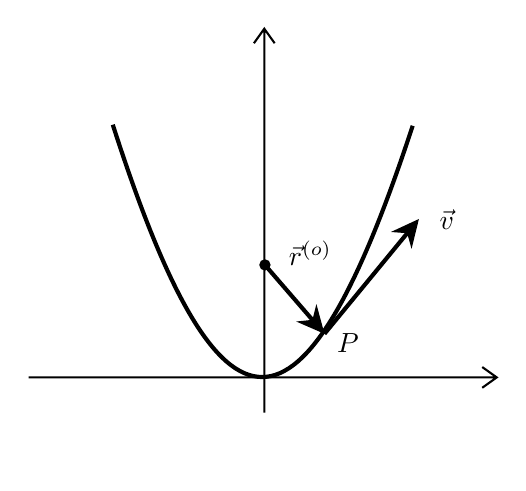
\begin{tikzpicture}[x=0.75pt,y=0.75pt,yscale=-1,xscale=1]
	%uncomment if require: \path (0,300); %set diagram left start at 0, and has height of 300

	% Plotting does not support converting to Tikz
	%Shape: Axis 2D [id:dp7726038513129663] 
	\draw  (128,195) -- (353.5,195)(241.5,27) -- (241.5,212) (346.5,190) -- (353.5,195) -- (346.5,200) (236.5,34) -- (241.5,27) -- (246.5,34)  ;
	%Shape: Circle [id:dp5040305763016306] 
	\draw  [fill={rgb, 255:red, 0; green, 0; blue, 0 }  ,fill opacity=1 ] (239.6,140.8) .. controls (239.6,139.58) and (240.58,138.6) .. (241.8,138.6) .. controls (243.02,138.6) and (244,139.58) .. (244,140.8) .. controls (244,142.02) and (243.02,143) .. (241.8,143) .. controls (240.58,143) and (239.6,142.02) .. (239.6,140.8) -- cycle ;
	%Straight Lines [id:da6870337422019563] 
	\draw [line width=1.5]    (241.8,140.8) -- (267.88,170.97) ;
	\draw [shift={(270.5,174)}, rotate = 229.16] [fill={rgb, 255:red, 0; green, 0; blue, 0 }  ][line width=0.08]  [draw opacity=0] (13.4,-6.43) -- (0,0) -- (13.4,6.44) -- (8.9,0) -- cycle    ;
	%Straight Lines [id:da9749674177874588] 
	\draw [line width=1.5]    (270.5,174) -- (313.46,121.76) ;
	\draw [shift={(316,118.67)}, rotate = 489.43] [fill={rgb, 255:red, 0; green, 0; blue, 0 }  ][line width=0.08]  [draw opacity=0] (13.4,-6.43) -- (0,0) -- (13.4,6.44) -- (8.9,0) -- cycle    ;
	%Curve Lines [id:da6365665117119264] 
	\draw [line width=1.5]    (168.5,73.25) .. controls (220.5,235.25) and (260,235.25) .. (313,73.75) ;

	% Text Node
	\draw (281.83,178.33) node    {$P$};
	% Text Node
	\draw (329.4,118.77) node    {$\vec{v}$};
	% Text Node
	\draw (263.67,134.97) node    {$\vec{r}^{( o)}$};

	\end{tikzpicture}
\end{figure}
\FloatBarrier

Il punto attorno al quale il punto materiale si muove prende il nome di \textbf{polo}. Il momento angolare è una grandezza vettoriale legata alla velocità del punto, in genere indicata con la lettera $\vec{L}$.
$\vec{L}^{(o)}$ si definisce come il prodotto vettoriale fra il vettore $\vec{r}_0$ e la quantità di moto del punto ed è sempre espresso rispetto al polo attorno a cui esso ruota.

\[
	\boxed{\vec{L}^{(o)}=\vec{r}\,^{(o)}\times m\vec{v}}
\]
È un vettore ortogonale al piano del moto, individuato da $\vec{r}\,^{(o)}$ e $\vec{v}$. Si chiama momento angolare perché è evidente che questa quantità posseduta dal punto materiale è non nulla tutte le volte che esso ha una velocità che presenta una componente ortogonale al vettore $\vec{r}\,^{(o)}$, è questa componente infatti che gli permette di ruotare attorno al polo. La componente parallela invece rappresenta la tendenza del punto ad avvicinarsi al polo $O$. Si osservi che il momento angolare si contrappone all'effetto che ha la quantità di moto, perché quest'ultima è sempre parallela alla traiettoria.

Così come la quantità di moto varia nel tempo sotto l'azione delle forze che agiscono sul punto $P$, analogamente ci sarà una quantità dinamica che fa variare nel tempo il momento angolare e che quindi entra in gioco quando una forza ha l'effetto di far ruotare il corpo. Se il punto materiale per qualche motivo è vincolato al polo $O$, tramite ad esempio un'asta rigida, l'effetto della forza $\vec{F}$ agente sul punto $P$ sarà che esso, non potendo traslare verso l'alto liberamente, ruota attorno al polo $O$. Per individuare questo effetto dinamico di rotazione, si definisce \textbf{momento della forza} rispetto al polo $O$ il prodotto vettoriale fra $\vec{r}\,^{(o)}$ e la forza $\vec{F}$. È quindi un vettore diretto ortogonalmente al piano formato dal vettore $\vec{r}\,^{(o)}$ e dal vettore $\vec{F}$. In seguito si studia come calcolare l'intensità del momento della forza in due modalità differenti.

\paragraph{Primo metodo} Si disegna una retta che ha la stessa direzione di $\vec{F}$ e si valuta la distanza assiale (angolo retto) fra il punto $P$ e questo asse, che ha la stessa direzione di $\vec{F}$. Questo tratto tratteggiato lo si chiama \textbf{braccio della forza}. Si ottiene che l'intensità del momento della forza è pari al prodotto fra l'intensità della forza e il suo braccio.

\begin{figure}[htpb]
	\centering

	\tikzset{every picture/.style={line width=0.75pt}} %set default line width to 0.75pt        

	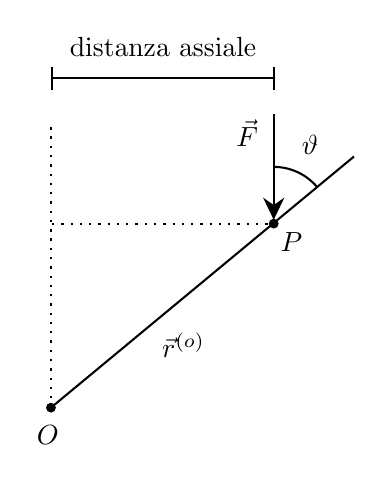
\begin{tikzpicture}[x=0.75pt,y=0.75pt,yscale=-1,xscale=1]
	%uncomment if require: \path (0,300); %set diagram left start at 0, and has height of 300

	%Straight Lines [id:da7921800429795998] 
	\draw    (167.5,242) -- (313.5,121) ;
	%Straight Lines [id:da5767628400815077] 
	\draw  [dash pattern={on 0.84pt off 2.51pt}]  (167.5,242) -- (167.5,103.67) ;
	%Straight Lines [id:da09563530908775442] 
	\draw    (274.83,148.5) -- (274.83,100.33) ;
	\draw [shift={(274.83,151.5)}, rotate = 270] [fill={rgb, 255:red, 0; green, 0; blue, 0 }  ][line width=0.08]  [draw opacity=0] (10.72,-5.15) -- (0,0) -- (10.72,5.15) -- (7.12,0) -- cycle    ;
	%Straight Lines [id:da48703129030454484] 
	\draw  [dash pattern={on 0.84pt off 2.51pt}]  (168,153.33) -- (274.83,153.33) ;
	%Shape: Circle [id:dp7102470019836413] 
	\draw  [fill={rgb, 255:red, 0; green, 0; blue, 0 }  ,fill opacity=1 ] (165.67,242) .. controls (165.67,240.99) and (166.49,240.17) .. (167.5,240.17) .. controls (168.51,240.17) and (169.33,240.99) .. (169.33,242) .. controls (169.33,243.01) and (168.51,243.83) .. (167.5,243.83) .. controls (166.49,243.83) and (165.67,243.01) .. (165.67,242) -- cycle ;
	%Shape: Circle [id:dp5463186831665952] 
	\draw  [fill={rgb, 255:red, 0; green, 0; blue, 0 }  ,fill opacity=1 ] (273,153.33) .. controls (273,152.32) and (273.82,151.5) .. (274.83,151.5) .. controls (275.85,151.5) and (276.67,152.32) .. (276.67,153.33) .. controls (276.67,154.35) and (275.85,155.17) .. (274.83,155.17) .. controls (273.82,155.17) and (273,154.35) .. (273,153.33) -- cycle ;
	%Shape: Arc [id:dp33721727159311543] 
	\draw  [draw opacity=0] (274.83,126) .. controls (274.83,126) and (274.83,126) .. (274.83,126) .. controls (283.24,126) and (290.76,129.8) .. (295.78,135.77) -- (274.83,153.33) -- cycle ; \draw   (274.83,126) .. controls (274.83,126) and (274.83,126) .. (274.83,126) .. controls (283.24,126) and (290.76,129.8) .. (295.78,135.77) ;
	%Straight Lines [id:da12096800312738543] 
	\draw    (168,83.33) -- (274.83,83.33) ;
	\draw [shift={(274.83,83.33)}, rotate = 180] [color={rgb, 255:red, 0; green, 0; blue, 0 }  ][line width=0.75]    (0,5.59) -- (0,-5.59)   ;
	\draw [shift={(168,83.33)}, rotate = 180] [color={rgb, 255:red, 0; green, 0; blue, 0 }  ][line width=0.75]    (0,5.59) -- (0,-5.59)   ;

	% Text Node
	\draw (231.33,212) node    {$\vec{r}^{( o)}$};
	% Text Node
	\draw (166,255.33) node    {$O$};
	% Text Node
	\draw (283.33,162.33) node    {$P$};
	% Text Node
	\draw (262,109.67) node    {$\vec{F}$};
	% Text Node
	\draw (292.33,115.33) node    {$\vartheta $};
	% Text Node
	\draw (221.5,68) node   [align=left] {distanza assiale};

	\end{tikzpicture}
\end{figure}
\FloatBarrier
A pari intensità della forza il momento è più grande se la distanza dal cardine è più lunga e c'è se la forza ha una componente ortogonale al raggio che identifica la posizione del punto $P$ rispetto al polo $O$.

\[
	\boxed{\norm{\vec{M}^{(o)}}= \norm{\vec{r}\,^{(o)}} \norm{\vec{F}} \sin\vartheta}
\]

In caso contrario, la forza ha solo l'effetto di trazione oppure di compressione, non ha momento e quindi non permette all'oggetto di ruotare intorno al polo.

Se si studia il moto del punto $P$ rispetto a un polo si potrà calcolare il momento di ognuna delle forze agenti su di esso. La somma di tutti questi momenti dà luogo alla \emph{risultante} dei momenti che stanno agendo sul punto materiale.

\begin{figure}[htpb]
	\centering

	\tikzset{every picture/.style={line width=0.75pt}} %set default line width to 0.75pt        

	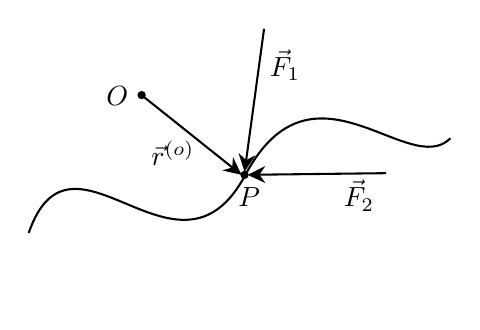
\begin{tikzpicture}[x=0.75pt,y=0.75pt,yscale=-0.8,xscale=0.8]
	%uncomment if require: \path (0,300); %set diagram left start at 0, and has height of 300

	%Curve Lines [id:da7301824126083205] 
	\draw    (69.5,155) .. controls (95.5,80) and (159.5,196) .. (200,120) .. controls (240.5,44) and (298.5,123) .. (323.5,98) ;
	%Shape: Circle [id:dp27186947828666264] 
	\draw  [fill={rgb, 255:red, 0; green, 0; blue, 0 }  ,fill opacity=1 ] (135.67,72) .. controls (135.67,70.99) and (136.49,70.17) .. (137.5,70.17) .. controls (138.51,70.17) and (139.33,70.99) .. (139.33,72) .. controls (139.33,73.01) and (138.51,73.83) .. (137.5,73.83) .. controls (136.49,73.83) and (135.67,73.01) .. (135.67,72) -- cycle ;
	%Straight Lines [id:da47132651835927253] 
	\draw    (195.32,118.13) -- (137.5,72) ;
	\draw [shift={(197.67,120)}, rotate = 218.58] [fill={rgb, 255:red, 0; green, 0; blue, 0 }  ][line width=0.08]  [draw opacity=0] (10.72,-5.15) -- (0,0) -- (10.72,5.15) -- (7.12,0) -- cycle    ;
	%Shape: Circle [id:dp27888495348889486] 
	\draw  [fill={rgb, 255:red, 0; green, 0; blue, 0 }  ,fill opacity=1 ] (197.67,120) .. controls (197.67,118.99) and (198.49,118.17) .. (199.5,118.17) .. controls (200.51,118.17) and (201.33,118.99) .. (201.33,120) .. controls (201.33,121.01) and (200.51,121.83) .. (199.5,121.83) .. controls (198.49,121.83) and (197.67,121.01) .. (197.67,120) -- cycle ;
	%Straight Lines [id:da3814471042063463] 
	\draw    (199.91,115.19) -- (211.25,32) ;
	\draw [shift={(199.5,118.17)}, rotate = 277.77] [fill={rgb, 255:red, 0; green, 0; blue, 0 }  ][line width=0.08]  [draw opacity=0] (10.72,-5.15) -- (0,0) -- (10.72,5.15) -- (7.12,0) -- cycle    ;
	%Straight Lines [id:da063971460239854] 
	\draw    (204.33,119.96) -- (284.75,119) ;
	\draw [shift={(201.33,120)}, rotate = 359.31] [fill={rgb, 255:red, 0; green, 0; blue, 0 }  ][line width=0.08]  [draw opacity=0] (10.72,-5.15) -- (0,0) -- (10.72,5.15) -- (7.12,0) -- cycle    ;

	% Text Node
	\draw (202.33,133.5) node    {$P$};
	% Text Node
	\draw (122.83,72.5) node    {$O$};
	% Text Node
	\draw (223.83,54) node    {$\vec{F}_{1}$};
	% Text Node
	\draw (268.33,132.5) node    {$\vec{F}_{2}$};
	% Text Node
	\draw (156.33,107) node    {$\vec{r}^{( o)}$};

	\end{tikzpicture}
\end{figure}
\FloatBarrier

\[
	\vec{M}_{\text{TOT}}=\vec{M}^{(o)}_1+\vec{M}^{(o)}_2= \vec{r}\,^{(o)} \times\vec{F}_1+\vec{r}\,^{(o)} \times \vec{F}_2= \vec{r}\,^{(o)} \times (\vec{F}_1+\vec{F}_2)
\]
È utile osservare che poiché il punto materiale è sempre lo stesso, quando si fa la somma si può applicare la proprietà distributiva. Ciò significa che è la stessa cosa sommare i singoli momenti o calcolare la risultante delle forze per poi calcolarne il momento.

\paragraph{Secondo metodo} Si comincia ricordando che le forze hanno l'effetto di far variare la quantità di moto:

\[
	\vec{F}=\frac{d(m\vec{v})}{dt}=\frac{d\vec{p}}{dt}
\]

Data questa espressione si prende il momento angolare e lo si deriva nel tempo.

\[
	\frac{d\vec{L}^{(o)}}{dt}=\frac{d(\vec{r}\,^{(o)}\times m\vec{v})}{dt}=\frac{d(\vec{r}\,^{(o)})}{dt}\times m\vec{v}+\underbrace{\vec{r}\,^{(o)}\times m\frac{d\vec{v}}{dt}}_{\vec{M}^{(o)}}
\]

Si comincia a vedere già meglio il legame fra l'effetto dinamico e la sua causa. $\frac{d\vec{r}}{dt}$ è la velocità del punto materiale osservato da un osservatore solidale al polo $O$. Ciò significa che tale termine non è altro che la velocità del punto $P$ meno la velocità di $O$.

\begin{gather*}
	\vec{v}_{\text{rel}}=\vec{v}-\vec{v}_0 \implies (\vec{v}-\vec{v}_0)\times m\vec{v}=\underbrace{\vec{v}\times m\vec{v}}_{=0}-\vec{v}_0 \times m\vec{v}=-\vec{v}_0 \times m\vec{v} \\
	\boxed{\frac{d\vec{L}^{(o)}}{dt} =-\vec{v}_0 \times m\vec{v}+ \vec{M}^{(o)}}
\end{gather*}

L'effetto dinamico che hanno questi momenti delle forze è quello di far variare nel tempo il momento angolare del punto. Questo risultato prende il nome di \textbf{teorema del momento angolare} del punto materiale ed è una diretta conseguenza della legge di Newton. Infatti, l'utilizzo del momento angolare e del momento della forza e delle loro proprietà, anche se rilevanti in alcuni casi specifici, non fornisce nessuna informazione che non sia già ricavabile direttamente da essa. Il termine aggiuntivo $-\vec{v}_0 \times m\vec{v}$ si annulla se il polo $O$ è fermo oppure se si muove con velocità parallela a quella del punto. In questo caso il teorema diventa:

\[
	\boxed{\vec{M}^{(o)}= \frac{d\vec{L}^{(o)}}{dt}}
\]

Se sul punto materiale agiscono delle forze che non generano momento, si trova come conseguenza il \textbf{principio di conservazione del momento angolare}:

\[
	\boxed{\vec{M}^{(o)}=0 \implies \vec{L}^{(o)}= \text{costante}}
\]

Si chiama in tal modo perché si può dimostrare che è un principio fondamentale che deriva dalla simmetria dello spazio nel tempo.

\section{Dinamica relativa}

Nel capitolo 2 si è determinato il legame sia in termini di velocità che di accelerazione fra ciò che rilevano l'osservatore assoluto e quello relativo. Vediamo come queste leggi si traducono sul moto di un corpo nel momento in cui su di esso agiscono delle forze. L'obbiettivo del paragrafo è quello di capire come l'osservatore dal sistema di riferimento mobile possa ancora usare i principi della dinamica newtoniana.
Il problema si presenta perché essi valgono solo se il sistema di riferimento è inerziale. In tal caso si ha:

\[
	\vec{F}=m\vec{a}
\]

dove le forze che compaiono a primo membro sono quelle reali, che derviano dalle interazioni fondamentali, e la risultante è proporzionale all'accelerazione misurata in quel sistema di riferimento. Si consideri ora un altro sistema di riferimento che si muove di moto traslatorio rettilineo uniforme rispetto ad un certo sistema inerziale. Si ha:

\[
	\vec{v}_{o'}=\text{costante} \quad \vec{a}_{o'}=0 \quad \vec{\omega}=0
\]

Dato che:

\[
	\vec{a}=\vec{a'}+\vec{a}_{o'}+\frac{d\vec{\omega}}{dt} \times \vec{r'}+\vec{\omega}\times (\vec{\omega} \times \vec{r'})+2\vec{\omega} \times \vec{v'} \quad \text{si ha} \quad \vec{a}=\vec{a'}
\]

Le accelerazioni di un punto misurate nei due sistemi di riferimento sono eguali. Se $a=0$ allora anche $a'=0$ e quindi anche il secondo sistema è inerziale. Questo porta a confermare il fatto che, definito un sistema di riferimento inerziale, tutti gli altri sistemi in moto rettilineo uniforme rispetto a questo sono anche essi inerziali. Per tali sistemi la legge di Newton si scrive allo stesso modo, ossia con gli stessi valori di $\vec{F}$ e $\vec{a}$. Conseguenza importante è che non è possibile stabilire tramite misure effettuate in questi diversi sistemi di riferimento, se uno di essi è in quiete o in moto. Si ricordi che tale situazione fisica viene descritta anche con il termine di relatività galileiana.

Tuttavia, se il moto del secondo sistema è accelerato rispetto al sistema inerziale, sia perché $a_{o'}$ o $\omega$ sono non nulle o per entrambe le ragioni, si osserva che la legge di Newton non è più valida, la forza vera che agisce sul punto considerato non è proporzionale alla sua accelerazione. Infatti, se $\vec{F}=m\vec{a}$ nel sistema inerziale, nel sistema mobile in moto accelerato non può sussistere la relazione $\vec{F}=m\vec{a'}$ perché $a$ e $a'$ sono diverse.
Quindi $F=ma'$ non è vera tutte le volte che esiste un'accelerazione di trascinamento e/o una di Coriolis. D'altra parte si può scrivere:

\[
	\vec{F}=m\vec{a}=m\vec{a}_{\text{rel}}+m\vec{a}_{\text{trasc}}+m\vec{a}_c
\]

Isolando l'accelerazione relativa:

\[
	m\vec{a}_{\text{rel}}=\vec{F} \underbrace{-m\vec{a}_{\text{trasc}}-m\vec{a}_c}_{\vec{F}_{\text{app}}}
\]

Il terimine $\vec{F}_{\text{app}}$ dimensionalmente è una forza e per questo motivo viene anche chiamato \textbf{forza apparente}. Quindi in un sistema di riferimento non inerziale il prodotto della massa del punto materiale per l'accelerazione misurata in quel sistema è eguale alla forza vera agente sul punto sommata a queste forze apparenti. Non si tratta di interazioni reali che effettivamente agiscono sul punto e che si possono ricondurre alle quattro interazioni fondamentali, ma costituiscono un termine correttivo che appare solo nel sistema non inerziale che permette di ricondursi a $F=ma'$ e vengono pertanto chiamate anche \textit{forze di inerzia}: grazie ad esse la seconda legge di Newton è rispettata.

\[
	\vec{F}_{\text{app}}=-m\vec{a}_{\text{trasc}}-m\vec{a}_c
\]

Si vede come allora sia possibile introdurre un secondo principio della dinamica modificato per i sistemi di riferimento non inerziali grazie a questo nuovo termine.

\[
	\vec{F}_{\text{app}}=(-m\vec{a}_{o'})+(-m\vec{\omega}\times \vec{\omega} \times \vec{r'})+(-m\vec{\alpha}\times\vec{r'})+(-2m\vec{\omega} \times \vec{v}_{\text{rel}})
\]

In particolare, la forza:

\[
	\vec{F}_{\text{cf}}=-m\vec{\omega}\times \vec{\omega} \times \vec{r'}
\]
è la cosiddetta \textbf{forza apparente centrifuga}. Il suo effetto può essere facilmente percepito quando ci si trova su un'automobile che percorre una rotatoria e si ha l'impressione di essere spinti verso l'esterno. Invece:

\[
	\vec{F}_c= -2m\vec{\omega} \times \vec{v}_{\text{rel}}
\]

prende il nome di \textbf{forza di Coriolis}.

\[
	\vec{F}+\vec{F}_{\text{app}}=m\vec{a}_{\text{rel}}
\]

Si noti in particolare come in un sistema accelerato $F=0$ non comporti $a=0$ e quindi l'osservazione di un moto rettilineo uniforme. Questo risultato giustifica il nome di sistema non inerziale per un sistema accelerato: in esso la legge di inerzia non vale.

\subsubsection{Moto di trascinamento rettilineo accelerato}

\paragraph{Primo esempio} Si supponga di avere un vagone di un treno che inizialmente si muove di moto uniforme rettilineo.

\begin{figure}[htpb]
	\centering

	\tikzset{every picture/.style={line width=0.75pt}} %set default line width to 0.75pt        

	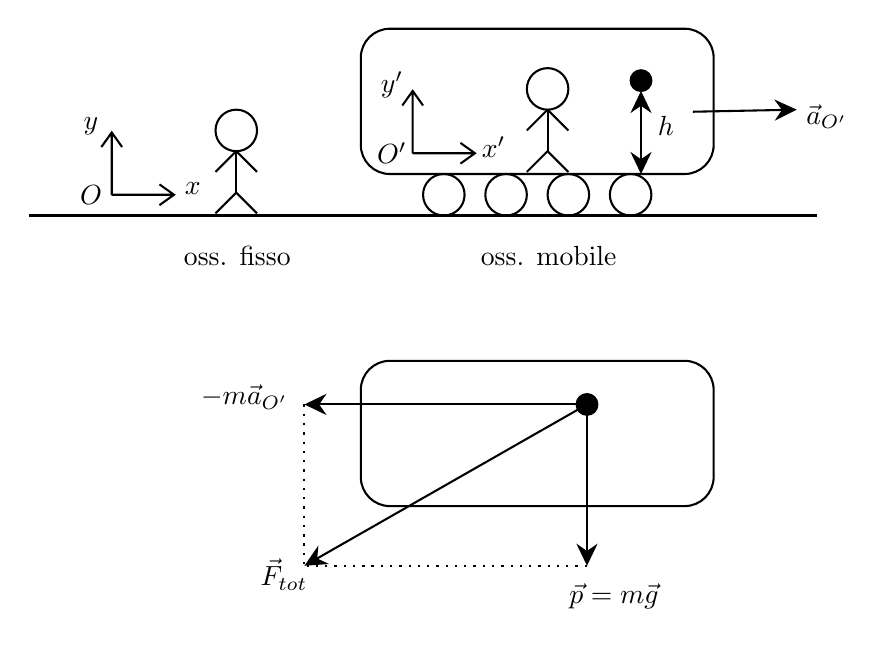
\begin{tikzpicture}[x=0.75pt,y=0.75pt,yscale=-1,xscale=1]
	%uncomment if require: \path (0,493); %set diagram left start at 0, and has height of 493

	%Straight Lines [id:da8845303315941491] 
	\draw    (50,190) -- (430,190) ;
	%Rounded Rect [id:dp5517065009785334] 
	\draw   (210,114) .. controls (210,106.27) and (216.27,100) .. (224,100) -- (366,100) .. controls (373.73,100) and (380,106.27) .. (380,114) -- (380,156) .. controls (380,163.73) and (373.73,170) .. (366,170) -- (224,170) .. controls (216.27,170) and (210,163.73) .. (210,156) -- cycle ;
	%Shape: Circle [id:dp28946861808735336] 
	\draw   (240,180) .. controls (240,174.48) and (244.48,170) .. (250,170) .. controls (255.52,170) and (260,174.48) .. (260,180) .. controls (260,185.52) and (255.52,190) .. (250,190) .. controls (244.48,190) and (240,185.52) .. (240,180) -- cycle ;
	%Shape: Circle [id:dp13801409799404407] 
	\draw   (270,180) .. controls (270,174.48) and (274.48,170) .. (280,170) .. controls (285.52,170) and (290,174.48) .. (290,180) .. controls (290,185.52) and (285.52,190) .. (280,190) .. controls (274.48,190) and (270,185.52) .. (270,180) -- cycle ;
	%Shape: Circle [id:dp29024094658021093] 
	\draw   (300,180) .. controls (300,174.48) and (304.48,170) .. (310,170) .. controls (315.52,170) and (320,174.48) .. (320,180) .. controls (320,185.52) and (315.52,190) .. (310,190) .. controls (304.48,190) and (300,185.52) .. (300,180) -- cycle ;
	%Shape: Circle [id:dp2732816373100859] 
	\draw   (330,180) .. controls (330,174.48) and (334.48,170) .. (340,170) .. controls (345.52,170) and (350,174.48) .. (350,180) .. controls (350,185.52) and (345.52,190) .. (340,190) .. controls (334.48,190) and (330,185.52) .. (330,180) -- cycle ;
	%Shape: Circle [id:dp9803871770324311] 
	\draw   (290,129) .. controls (290,123.48) and (294.48,119) .. (300,119) .. controls (305.52,119) and (310,123.48) .. (310,129) .. controls (310,134.52) and (305.52,139) .. (300,139) .. controls (294.48,139) and (290,134.52) .. (290,129) -- cycle ;
	%Straight Lines [id:da5918357181478389] 
	\draw    (300,159) -- (300,139) ;
	%Straight Lines [id:da8644803390899314] 
	\draw    (310,169) -- (300,159) ;
	%Straight Lines [id:da9988000045948477] 
	\draw    (310,149) -- (300,139) ;
	%Straight Lines [id:da5227285209954715] 
	\draw    (290,149) -- (300,139) ;
	%Straight Lines [id:da72039255595026] 
	\draw    (290,169) -- (300,159) ;

	%Shape: Circle [id:dp7254243014258992] 
	\draw   (140,149) .. controls (140,143.48) and (144.48,139) .. (150,139) .. controls (155.52,139) and (160,143.48) .. (160,149) .. controls (160,154.52) and (155.52,159) .. (150,159) .. controls (144.48,159) and (140,154.52) .. (140,149) -- cycle ;
	%Straight Lines [id:da3738111513126945] 
	\draw    (150,179) -- (150,159) ;
	%Straight Lines [id:da9266705565337741] 
	\draw    (160,189) -- (150,179) ;
	%Straight Lines [id:da549874811572632] 
	\draw    (160,169) -- (150,159) ;
	%Straight Lines [id:da4835894229807174] 
	\draw    (140,169) -- (150,159) ;
	%Straight Lines [id:da9048075753546523] 
	\draw    (140,189) -- (150,179) ;

	%Shape: Axis 2D [id:dp683490375288136] 
	\draw  (90,180) -- (120,180)(90,150) -- (90,180) -- cycle (113,175) -- (120,180) -- (113,185) (85,157) -- (90,150) -- (95,157)  ;
	%Shape: Axis 2D [id:dp01355233214226792] 
	\draw  (235,160) -- (265,160)(235,130) -- (235,160) -- cycle (258,155) -- (265,160) -- (258,165) (230,137) -- (235,130) -- (240,137)  ;
	%Straight Lines [id:da6449047403936963] 
	\draw    (370,140) -- (417,139.06) ;
	\draw [shift={(420,139)}, rotate = 538.85] [fill={rgb, 255:red, 0; green, 0; blue, 0 }  ][line width=0.08]  [draw opacity=0] (10.72,-5.15) -- (0,0) -- (10.72,5.15) -- (7.12,0) -- cycle    ;
	%Shape: Circle [id:dp6949534200545615] 
	\draw  [fill={rgb, 255:red, 0; green, 0; blue, 0 }  ,fill opacity=1 ] (340,125) .. controls (340,122.24) and (342.24,120) .. (345,120) .. controls (347.76,120) and (350,122.24) .. (350,125) .. controls (350,127.76) and (347.76,130) .. (345,130) .. controls (342.24,130) and (340,127.76) .. (340,125) -- cycle ;
	%Straight Lines [id:da7649546918616734] 
	\draw    (345,133) -- (345,167) ;
	\draw [shift={(345,170)}, rotate = 270] [fill={rgb, 255:red, 0; green, 0; blue, 0 }  ][line width=0.08]  [draw opacity=0] (10.72,-5.15) -- (0,0) -- (10.72,5.15) -- (7.12,0) -- cycle    ;
	\draw [shift={(345,130)}, rotate = 90] [fill={rgb, 255:red, 0; green, 0; blue, 0 }  ][line width=0.08]  [draw opacity=0] (10.72,-5.15) -- (0,0) -- (10.72,5.15) -- (7.12,0) -- cycle    ;
	%Rounded Rect [id:dp6299281142169286] 
	\draw   (210,274) .. controls (210,266.27) and (216.27,260) .. (224,260) -- (366,260) .. controls (373.73,260) and (380,266.27) .. (380,274) -- (380,316) .. controls (380,323.73) and (373.73,330) .. (366,330) -- (224,330) .. controls (216.27,330) and (210,323.73) .. (210,316) -- cycle ;
	%Straight Lines [id:da4399120364271609] 
	\draw    (318.98,281.02) -- (185.82,281.02) ;
	\draw [shift={(182.82,281.02)}, rotate = 360] [fill={rgb, 255:red, 0; green, 0; blue, 0 }  ][line width=0.08]  [draw opacity=0] (10.72,-5.15) -- (0,0) -- (10.72,5.15) -- (7.12,0) -- cycle    ;
	%Straight Lines [id:da11021083557463185] 
	\draw    (318.98,281.02) -- (318.98,355.75) ;
	\draw [shift={(318.98,358.75)}, rotate = 270] [fill={rgb, 255:red, 0; green, 0; blue, 0 }  ][line width=0.08]  [draw opacity=0] (10.72,-5.15) -- (0,0) -- (10.72,5.15) -- (7.12,0) -- cycle    ;
	%Straight Lines [id:da5241271764093178] 
	\draw  [dash pattern={on 0.84pt off 2.51pt}]  (318.98,358.75) -- (182.82,358.75) ;
	%Straight Lines [id:da06747514242420771] 
	\draw  [dash pattern={on 0.84pt off 2.51pt}]  (182.82,281.02) -- (182.82,358.75) ;
	%Straight Lines [id:da37342175067776906] 
	\draw    (318.98,281.02) -- (185.42,357.26) ;
	\draw [shift={(182.82,358.75)}, rotate = 330.28] [fill={rgb, 255:red, 0; green, 0; blue, 0 }  ][line width=0.08]  [draw opacity=0] (10.72,-5.15) -- (0,0) -- (10.72,5.15) -- (7.12,0) -- cycle    ;
	%Shape: Circle [id:dp3288407095021495] 
	\draw  [fill={rgb, 255:red, 0; green, 0; blue, 0 }  ,fill opacity=1 ] (313.98,281.02) .. controls (313.98,278.26) and (316.21,276.02) .. (318.98,276.02) .. controls (321.74,276.02) and (323.98,278.26) .. (323.98,281.02) .. controls (323.98,283.79) and (321.74,286.02) .. (318.98,286.02) .. controls (316.21,286.02) and (313.98,283.79) .. (313.98,281.02) -- cycle ;

	% Text Node
	\draw (129,177) node    {$x$};
	% Text Node
	\draw (80,147) node    {$y$};
	% Text Node
	\draw (80,180) node    {$O$};
	% Text Node
	\draw (274,157) node    {$x'$};
	% Text Node
	\draw (225,127) node    {$y'$};
	% Text Node
	\draw (225,160) node    {$O'$};
	% Text Node
	\draw (434.5,142.5) node    {$\vec{a}_{O'}$};
	% Text Node
	\draw (150.5,209.5) node   [align=left] {oss. fisso};
	% Text Node
	\draw (300.5,209.5) node   [align=left] {oss. mobile};
	% Text Node
	\draw (357,147) node    {$h$};
	% Text Node
	\draw (154,277.5) node    {$-m\vec{a}_{O'}$};
	% Text Node
	\draw (332,373.5) node    {$\vec{p} =m\vec{g}$};
	% Text Node
	\draw (173,363) node    {$\vec{F}_{tot}$};

	\end{tikzpicture}
\end{figure}
\FloatBarrier
All'istante $t_0$ esso viene accelerato in avanti con una certa accelerazione $\vec{a}_{O'}$. Si considerino successivamente un osservatore fisso fuori dal treno e uno mobile solidale ad esso e un oggetto di massa $m$ che si trova sollevato a una certa quota $h$ all'interno di un vagone. Nell'istante in cui il treno accelera esso viene lasciato libero di cadere. Si è interessati a capire quale sia il moto di caduta dell'oggetto visto da $O$ e da $O'$.

Negli istanti successivi a $t_0$ il corpo è soltanto sottoposto alla forza di gravità. Tuttavia il treno mentre esso cade si sposta più avanti così che l'oggetto tocca il pavimento del vagone più indietro rispetto a $O'$, di uno spostamento $d$. L'osservatore $O'$ rileverà quindi un moto di caduta parabolico. Dovrebbero esserci delle forze che giustificano questo moto, ma l'unica forza esistente è la forza peso. Bisogna quindi considerare l'esistenza di una forza apparente diretta verso sinistra parallela all'asse $x$. La forza apparente e la forza peso si sommano vettorialmente.

L'osservatore $O$ invece osserverà un normale moto di caduta verticale uniformemente accelerato.

\paragraph{Secondo esempio} Si immagini la stessa situazione vista nell'esempio precedente, ma al posto di avere un oggetto che viene lasciato cadere si ha un corpo appoggiato su un tavolo. Si trascuri l'effetto dell'attrito. Dal punto di vista dell'osservatore esterno, l'oggetto rimane fermo, $O'$ invece percepisce l'oggetto venire verso di sé. Per spiegare questo il cervello introduce una forza apparente.

\begin{figure}[htpb]
	\centering

	\tikzset{every picture/.style={line width=0.75pt}} %set default line width to 0.75pt        

	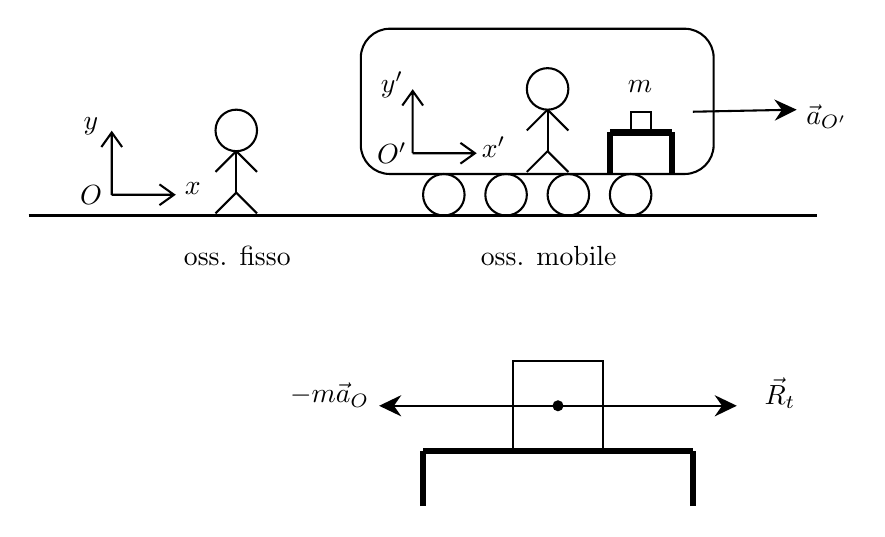
\begin{tikzpicture}[x=0.75pt,y=0.75pt,yscale=-1,xscale=1]
	%uncomment if require: \path (0,383); %set diagram left start at 0, and has height of 383

	%Straight Lines [id:da7481618489533346] 
	\draw    (50,150) -- (430,150) ;
	%Rounded Rect [id:dp5667741041831242] 
	\draw   (210,74) .. controls (210,66.27) and (216.27,60) .. (224,60) -- (366,60) .. controls (373.73,60) and (380,66.27) .. (380,74) -- (380,116) .. controls (380,123.73) and (373.73,130) .. (366,130) -- (224,130) .. controls (216.27,130) and (210,123.73) .. (210,116) -- cycle ;
	%Shape: Circle [id:dp2747437249820368] 
	\draw   (240,140) .. controls (240,134.48) and (244.48,130) .. (250,130) .. controls (255.52,130) and (260,134.48) .. (260,140) .. controls (260,145.52) and (255.52,150) .. (250,150) .. controls (244.48,150) and (240,145.52) .. (240,140) -- cycle ;
	%Shape: Circle [id:dp4412374085386952] 
	\draw   (270,140) .. controls (270,134.48) and (274.48,130) .. (280,130) .. controls (285.52,130) and (290,134.48) .. (290,140) .. controls (290,145.52) and (285.52,150) .. (280,150) .. controls (274.48,150) and (270,145.52) .. (270,140) -- cycle ;
	%Shape: Circle [id:dp34192828888252835] 
	\draw   (300,140) .. controls (300,134.48) and (304.48,130) .. (310,130) .. controls (315.52,130) and (320,134.48) .. (320,140) .. controls (320,145.52) and (315.52,150) .. (310,150) .. controls (304.48,150) and (300,145.52) .. (300,140) -- cycle ;
	%Shape: Circle [id:dp9465454617396569] 
	\draw   (330,140) .. controls (330,134.48) and (334.48,130) .. (340,130) .. controls (345.52,130) and (350,134.48) .. (350,140) .. controls (350,145.52) and (345.52,150) .. (340,150) .. controls (334.48,150) and (330,145.52) .. (330,140) -- cycle ;
	%Shape: Circle [id:dp5345063228583655] 
	\draw   (290,89) .. controls (290,83.48) and (294.48,79) .. (300,79) .. controls (305.52,79) and (310,83.48) .. (310,89) .. controls (310,94.52) and (305.52,99) .. (300,99) .. controls (294.48,99) and (290,94.52) .. (290,89) -- cycle ;
	%Straight Lines [id:da9418121610599619] 
	\draw    (300,119) -- (300,99) ;
	%Straight Lines [id:da4873352074315478] 
	\draw    (310,129) -- (300,119) ;
	%Straight Lines [id:da2265861890506471] 
	\draw    (310,109) -- (300,99) ;
	%Straight Lines [id:da4267121758287853] 
	\draw    (290,109) -- (300,99) ;
	%Straight Lines [id:da3908971786394406] 
	\draw    (290,129) -- (300,119) ;

	%Shape: Circle [id:dp1205389278798743] 
	\draw   (140,109) .. controls (140,103.48) and (144.48,99) .. (150,99) .. controls (155.52,99) and (160,103.48) .. (160,109) .. controls (160,114.52) and (155.52,119) .. (150,119) .. controls (144.48,119) and (140,114.52) .. (140,109) -- cycle ;
	%Straight Lines [id:da1777074619744483] 
	\draw    (150,139) -- (150,119) ;
	%Straight Lines [id:da8202026608698005] 
	\draw    (160,149) -- (150,139) ;
	%Straight Lines [id:da3057970641206704] 
	\draw    (160,129) -- (150,119) ;
	%Straight Lines [id:da09311157856084074] 
	\draw    (140,129) -- (150,119) ;
	%Straight Lines [id:da009624285579875158] 
	\draw    (140,149) -- (150,139) ;

	%Shape: Axis 2D [id:dp8662876823902428] 
	\draw  (90,140) -- (120,140)(90,110) -- (90,140) -- cycle (113,135) -- (120,140) -- (113,145) (85,117) -- (90,110) -- (95,117)  ;
	%Shape: Axis 2D [id:dp5231104317813651] 
	\draw  (235,120) -- (265,120)(235,90) -- (235,120) -- cycle (258,115) -- (265,120) -- (258,125) (230,97) -- (235,90) -- (240,97)  ;
	%Straight Lines [id:da7998457648446491] 
	\draw    (370,100) -- (417,99.06) ;
	\draw [shift={(420,99)}, rotate = 538.85] [fill={rgb, 255:red, 0; green, 0; blue, 0 }  ][line width=0.08]  [draw opacity=0] (10.72,-5.15) -- (0,0) -- (10.72,5.15) -- (7.12,0) -- cycle    ;
	%Straight Lines [id:da08530829866443712] 
	\draw    (305,241.67) -- (221.84,241.67) ;
	\draw [shift={(218.84,241.67)}, rotate = 360] [fill={rgb, 255:red, 0; green, 0; blue, 0 }  ][line width=0.08]  [draw opacity=0] (10.72,-5.15) -- (0,0) -- (10.72,5.15) -- (7.12,0) -- cycle    ;
	%Shape: Rectangle [id:dp12171107723467856] 
	\draw   (340,100) -- (350,100) -- (350,110) -- (340,110) -- cycle ;
	%Straight Lines [id:da017961366152073666] 
	\draw [line width=2.25]    (330,110) -- (360,110) ;
	%Straight Lines [id:da6976251861981426] 
	\draw [line width=2.25]    (330,130) -- (330,110) ;
	%Straight Lines [id:da5278964740683598] 
	\draw [line width=2.25]    (360,130) -- (360,110) ;
	%Shape: Rectangle [id:dp971974753281907] 
	\draw   (283.33,220) -- (326.67,220) -- (326.67,263.33) -- (283.33,263.33) -- cycle ;
	%Straight Lines [id:da6316657209710219] 
	\draw [line width=2.25]    (240,263.33) -- (370,263.33) ;
	%Straight Lines [id:da3197068016741924] 
	\draw [line width=2.25]    (240,290) -- (240,263.33) ;
	%Straight Lines [id:da15778515861977183] 
	\draw [line width=2.25]    (370,290) -- (370,263.33) ;
	%Straight Lines [id:da7707290971716076] 
	\draw    (388.16,241.67) -- (305,241.67) ;
	\draw [shift={(391.16,241.67)}, rotate = 180] [fill={rgb, 255:red, 0; green, 0; blue, 0 }  ][line width=0.08]  [draw opacity=0] (10.72,-5.15) -- (0,0) -- (10.72,5.15) -- (7.12,0) -- cycle    ;
	%Shape: Circle [id:dp8261532738782928] 
	\draw  [fill={rgb, 255:red, 0; green, 0; blue, 0 }  ,fill opacity=1 ] (302.88,241.67) .. controls (302.88,240.49) and (303.83,239.54) .. (305,239.54) .. controls (306.17,239.54) and (307.13,240.49) .. (307.13,241.67) .. controls (307.13,242.84) and (306.17,243.79) .. (305,243.79) .. controls (303.83,243.79) and (302.88,242.84) .. (302.88,241.67) -- cycle ;

	% Text Node
	\draw (129,137) node    {$x$};
	% Text Node
	\draw (80,107) node    {$y$};
	% Text Node
	\draw (80,140) node    {$O$};
	% Text Node
	\draw (274,117) node    {$x'$};
	% Text Node
	\draw (225,87) node    {$y'$};
	% Text Node
	\draw (225,120) node    {$O'$};
	% Text Node
	\draw (434.5,102.5) node    {$\vec{a}_{O'}$};
	% Text Node
	\draw (150.5,169.5) node   [align=left] {oss. fisso};
	% Text Node
	\draw (300.5,169.5) node   [align=left] {oss. mobile};
	% Text Node
	\draw (344.5,88) node    {$m$};
	% Text Node
	\draw (195,236.5) node    {$-m\vec{a}_{O}$};
	% Text Node
	\draw (412,235.5) node    {$\vec{R}_{t}$};

	\end{tikzpicture}
\end{figure}
\FloatBarrier
Si immagini ora che fra l'oggetto appoggiato e il tavolo ci sia un attrito statico che mantiene l'oggetto fermo. La forza di attrito bilancia la forza apparente e quindi l'osservatore al di fuori vede l'oggetto accelerare in avanti con accelerazione $\vec{a}_{O'}$. La forza di attrito è quella che permette al corpo di andare in avanti. La forza reale $R_t$ ha una sua reazione che si dovrà applicare sul tavolo (per la terza legge della dinamica), mentre la forza apparente non ha alcuna reazione su quest'ultimo perché non è una vera forza.

\subsubsection{Moto di trascinamento rotatorio uniforme}

\paragraph{Primo esempio} Si immagini di avere una giostra che sta ruotando intorno al proprio asse di rotazione con velocità angolare costante. Un bambino $A$ è seduto al centro della giostra e un altro $B$ è in piedi davanti a lui al lato opposto. $A$ vuole lanciare un pallone al suo amico.

\begin{figure}[htpb]
	\centering

	\tikzset{every picture/.style={line width=0.75pt}} %set default line width to 0.75pt        

	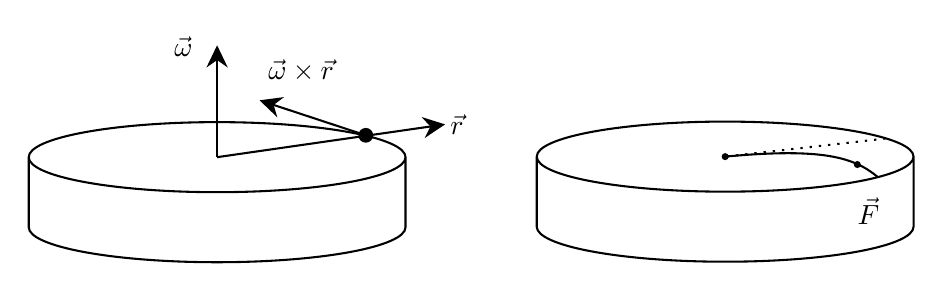
\begin{tikzpicture}[x=0.75pt,y=0.75pt,yscale=-1,xscale=1]
	%uncomment if require: \path (0,417); %set diagram left start at 0, and has height of 417

	%Shape: Can [id:dp1996235754689646] 
	\draw   (304.74,186.82) -- (304.74,220.57) .. controls (304.74,229.89) and (264.1,237.44) .. (213.96,237.44) .. controls (163.83,237.44) and (123.19,229.89) .. (123.19,220.57) -- (123.19,186.82) .. controls (123.19,177.5) and (163.83,169.94) .. (213.96,169.94) .. controls (264.1,169.94) and (304.74,177.5) .. (304.74,186.82) .. controls (304.74,196.14) and (264.1,203.69) .. (213.96,203.69) .. controls (163.83,203.69) and (123.19,196.14) .. (123.19,186.82) ;
	%Straight Lines [id:da1965995670183247] 
	\draw    (213.96,135.92) -- (213.96,186.82) ;
	\draw [shift={(213.96,132.92)}, rotate = 90] [fill={rgb, 255:red, 0; green, 0; blue, 0 }  ][line width=0.08]  [draw opacity=0] (10.72,-5.15) -- (0,0) -- (10.72,5.15) -- (7.12,0) -- cycle    ;
	%Straight Lines [id:da6025617807584005] 
	\draw    (320.82,171.46) -- (213.96,186.82) ;
	\draw [shift={(323.79,171.03)}, rotate = 171.82] [fill={rgb, 255:red, 0; green, 0; blue, 0 }  ][line width=0.08]  [draw opacity=0] (10.72,-5.15) -- (0,0) -- (10.72,5.15) -- (7.12,0) -- cycle    ;
	%Straight Lines [id:da686534953691958] 
	\draw    (237.27,160.36) -- (285.59,176.29) ;
	\draw [shift={(234.42,159.42)}, rotate = 18.25] [fill={rgb, 255:red, 0; green, 0; blue, 0 }  ][line width=0.08]  [draw opacity=0] (10.72,-5.15) -- (0,0) -- (10.72,5.15) -- (7.12,0) -- cycle    ;
	%Shape: Ellipse [id:dp14957173649018563] 
	\draw  [fill={rgb, 255:red, 0; green, 0; blue, 0 }  ,fill opacity=1 ] (282.55,176.29) .. controls (282.55,174.61) and (283.91,173.25) .. (285.59,173.25) .. controls (287.27,173.25) and (288.64,174.61) .. (288.64,176.29) .. controls (288.64,177.97) and (287.27,179.33) .. (285.59,179.33) .. controls (283.91,179.33) and (282.55,177.97) .. (282.55,176.29) -- cycle ;
	%Shape: Can [id:dp8485531513937126] 
	\draw   (549.5,186.56) -- (549.5,220.31) .. controls (549.5,229.63) and (508.86,237.19) .. (458.72,237.19) .. controls (408.59,237.19) and (367.95,229.63) .. (367.95,220.31) -- (367.95,186.56) .. controls (367.95,177.24) and (408.59,169.68) .. (458.72,169.68) .. controls (508.86,169.68) and (549.5,177.24) .. (549.5,186.56) .. controls (549.5,195.88) and (508.86,203.44) .. (458.72,203.44) .. controls (408.59,203.44) and (367.95,195.88) .. (367.95,186.56) ;
	%Straight Lines [id:da34569188456151245] 
	\draw  [dash pattern={on 0.84pt off 2.51pt}]  (536.03,177.85) -- (458.72,186.56) ;
	%Shape: Ellipse [id:dp5567109055251096] 
	\draw  [fill={rgb, 255:red, 0; green, 0; blue, 0 }  ,fill opacity=1 ] (457.57,186.56) .. controls (457.57,185.92) and (458.08,185.4) .. (458.72,185.4) .. controls (459.36,185.4) and (459.88,185.92) .. (459.88,186.56) .. controls (459.88,187.2) and (459.36,187.72) .. (458.72,187.72) .. controls (458.08,187.72) and (457.57,187.2) .. (457.57,186.56) -- cycle ;
	%Curve Lines [id:da8168874457095212] 
	\draw    (458.72,186.56) .. controls (505.54,182.2) and (520.78,186.83) .. (532.22,196.36) ;
	%Shape: Ellipse [id:dp4186108813920151] 
	\draw  [fill={rgb, 255:red, 0; green, 0; blue, 0 }  ,fill opacity=1 ] (521.26,190.37) .. controls (521.26,189.73) and (521.78,189.21) .. (522.42,189.21) .. controls (523.06,189.21) and (523.57,189.73) .. (523.57,190.37) .. controls (523.57,191.01) and (523.06,191.53) .. (522.42,191.53) .. controls (521.78,191.53) and (521.26,191.01) .. (521.26,190.37) -- cycle ;

	% Text Node
	\draw (329.51,171.3) node    {$\vec{r}$};
	% Text Node
	\draw (197.77,133.64) node    {$\vec{\omega }$};
	% Text Node
	\draw (254.43,145.16) node    {$\vec{\omega } \times \vec{r}$};
	% Text Node
	\draw (527.82,212.7) node    {$\vec{F}$};

	\end{tikzpicture}
\end{figure}
\FloatBarrier
La velocità lineare non è uguale per i punti sulla giostra: il bambino al centro gira su se stesso, ha velocità lineare pari a $0$, mentre $B$ ha una certa velocità lineare non nulla. Come conseguenza di ciò quando il pallone è arrivato al punto $x$, il bambino $B$ intanto si è spostato. La traiettoria che percepisce l'osservatore assoluto è dritta che cade verso il basso. L'osservatore che ruota osserva invece una traiettoria che curva come in figura.

\paragraph{Secondo esempio} Si consideri ora il sistema inerziale $O$ costituito da una coppia di assi cartesiani $x, y$ posti su un piano orizzontale, e il sistema non inerziale $O'$ costituito da un'altra coppia di assi $x', y'$ con la stessa origine e nello stesso piano, ruotanti con velocità angolare costante $\omega$. Si può ad esempio assumere gli assi $x', y'$ solidali ad un disco posto nel piano $x, y$ che ruota rispetto ad un asse passante per il suo centro e ortogonale al piano $x, y$. Se si pone un punto materiale sul disco, con attrito nullo, il punto $P$ rimane fermo mentre il disco gira sotto di esso. Se $P$ lasciasse una traccia, si osserverebbe una circonferenza di raggio $R$, con centro nell'origine comune dei due sistemi. Per l'osservatore $O$ il punto è in quiete, mentre per quello rotante $O'$ descrive un moto circolare uniforme. $O'$ deve allora ipotizzare che agiscano delle forze (centrifuga e di Coriolis) le quali, combinandosi, comunicano al punto l'accelerazione $a'$. Rimane il problema dell'origine di queste forze.

Si ipotizzi ore di legare con un filo il punto all'asse di rotazione e di dargli una velocità di modulo $\omega r$ in modo tale che ruoti con la stessa velocità del punto del disco su cui si trova. La situazione è opposta a quella precedente: per $O$ il punto descrive un moto circolare uniforme sotto l'azione della tensione del filo, mentre $O'$ vede il punto fermo. Esso è costretto a supporre che sul punto agisca una forza diretta verso l'esterno, che chiama forza centrifuga, bilanciata dalla tensione del filo. Per verificare l'ipotesi $O'$ traccia un segno radiale sul disco e recide il legame tra il punto e l'origine degli assi, immaginando di vederlo allontanarsi radialmente sotto l'azione della forza centrifuga, in quanto è stata annullata la forza esercitata dal filo. In effetti $O'$ osserva un moto del punto materiale, però lungo una traiettoria curvilinea, e deve quindi ammettere, come già fatto, che sui punti in moto nel suo sistema di rifermo, agisca un'altra forza che non si manifesta quando sono in quiete, la forza di Coriolis. Nel sistema inerziale invece il punto materiale all'istante in cui viene lasciato libero inizia a muoversi di moto rettilineo uniforme con direzione tangente alla circonferenza nella posizione in cui avviene il distacco dal vincolo.  In un sistema rotante è corretto attribuire alla forza centrifuga la tendenza allo spostamento radiale verso l'esterno e alla forza di Coriolis l'incurvamento della traiettoria osservata. La cosa importante è avere ben chiara l'origine di tali forze apparenti e utilizzarle correttamente dove appropriato e non estendere la loro esistenza ai sistemi inerziali.

\subsubsection{Il moto rispetto alla Terra}

\paragraph{Forza di Coriolis} Si trova discorso analogo a quello fatto in precedenza considerando gli effetti della rotazione della Terra intorno al proprio asse. Si ha di nuovo un effetto dovuto al fatto che un punto $P$ sopra la Terra si muove con una certa $\omega$ che è la stessa per tutti i punti del pianeta ma con una velocità lineare, diretta come il parallelo, che è massima all'equatore e va a via via diminuendo lungo i poli. Questo fatto fa si che, ad esempio, un osservatore posto su un aereo che si muove da sud a nord percepisca una deviazione verso destra. Esso infatti finisce per trovarsi su punti che via via si stanno muovendo con velocità lineare inferiore: questo è di nuovo un effetto della forza di Coriolis. Essa è tangente al parallelo e diretta verso est e il suo effetto a pari velocità relativa dell'aereo, è tanto più intenso quanto più ci si sposta ai poli, perché diventa sempre più importante la componente della velocità relativa diretta ortogonalmente a $\vec{\omega}$.

\paragraph{Forza centrifuga} Si immagini ora di avere un filo a piombo sospeso lungo la verticale. A causa dell'effetto della rotazione terrestre non si vede il lampadario diretto lungo la direzione dell'accelerazione di gravità. Sull'oggetto agisce la forza peso compensata dalla tensione del filo. Un osservatore assoluto vede il filo a piombo che ha la direzione che congiunge il punto materiale con il centro della Terra. L'osservatore mobile dovrà introdurre delle forze apparenti. L'unica in questo caso è la forza centrifuga, che sarà:

\[
	\vec{F}_{\text{cf}}=-m \vec{\omega} \times (\vec{\omega} \times \vec{r'} ) \implies \norm{\vec{F}_{\text{cf}}}=m\omega^2 R_t \cos\lambda
\]

Sulla Terra si percepisce un'accelerazione complessiva in modo tale che il filo a piombo non punterà veramente verso il centro della Terra ma è leggermente inclinato verso sud nell'emisfero boreale, verso Nord nell'emisfero australe (verso l'equatore).

\begin{figure}[htpb]
	\centering

	\tikzset{every picture/.style={line width=0.75pt}} %set default line width to 0.75pt        

	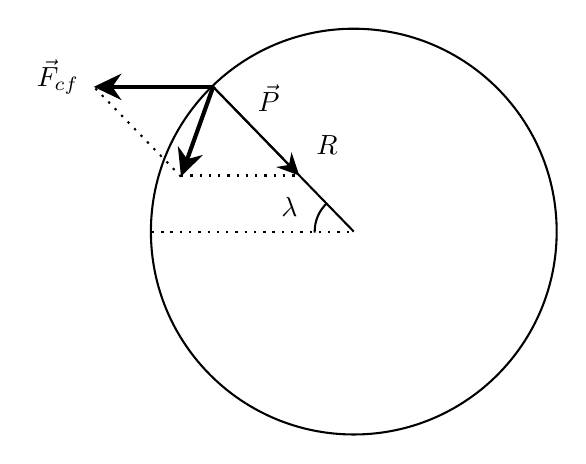
\begin{tikzpicture}[x=0.75pt,y=0.75pt,yscale=-1,xscale=1]
	%uncomment if require: \path (0,300); %set diagram left start at 0, and has height of 300

	%Shape: Circle [id:dp7489150544907581] 
	\draw   (156,146.75) .. controls (156,92.76) and (199.76,49) .. (253.75,49) .. controls (307.74,49) and (351.5,92.76) .. (351.5,146.75) .. controls (351.5,200.74) and (307.74,244.5) .. (253.75,244.5) .. controls (199.76,244.5) and (156,200.74) .. (156,146.75) -- cycle ;
	%Straight Lines [id:da6254894909113031] 
	\draw [line width=1.5]    (186,77) -- (132.5,77) ;
	\draw [shift={(128.5,77)}, rotate = 360] [fill={rgb, 255:red, 0; green, 0; blue, 0 }  ][line width=0.08]  [draw opacity=0] (13.4,-6.43) -- (0,0) -- (13.4,6.44) -- (8.9,0) -- cycle    ;
	%Straight Lines [id:da12818472298876005] 
	\draw  [dash pattern={on 0.84pt off 2.51pt}]  (156.5,146.75) -- (253.75,146.75) ;
	%Straight Lines [id:da8541133725441592] 
	\draw    (253.75,146.75) -- (186,77) ;
	%Shape: Boxed Line [id:dp3732214130705598] 
	\draw    (225.41,117.57) -- (186,77) ;
	\draw [shift={(227.5,119.73)}, rotate = 225.83] [fill={rgb, 255:red, 0; green, 0; blue, 0 }  ][line width=0.08]  [draw opacity=0] (10.72,-5.15) -- (0,0) -- (10.72,5.15) -- (7.12,0) -- cycle    ;
	%Straight Lines [id:da3181484584982588] 
	\draw  [dash pattern={on 0.84pt off 2.51pt}]  (170.5,119.73) -- (227.5,119.73) ;
	%Shape: Boxed Line [id:dp8534461017405279] 
	\draw  [dash pattern={on 0.84pt off 2.51pt}]  (170.5,120.24) -- (128.5,77) ;
	%Straight Lines [id:da7939485633198569] 
	\draw [line width=1.5]    (186,77) -- (171.85,116.47) ;
	\draw [shift={(170.5,120.24)}, rotate = 289.72] [fill={rgb, 255:red, 0; green, 0; blue, 0 }  ][line width=0.08]  [draw opacity=0] (13.4,-6.43) -- (0,0) -- (13.4,6.44) -- (8.9,0) -- cycle    ;
	%Shape: Arc [id:dp7184725777533214] 
	\draw  [draw opacity=0] (234.91,147.27) .. controls (234.9,147.1) and (234.9,146.92) .. (234.9,146.75) .. controls (234.9,141.27) and (237.24,136.34) .. (240.97,132.89) -- (253.75,146.75) -- cycle ; \draw   (234.91,147.27) .. controls (234.9,147.1) and (234.9,146.92) .. (234.9,146.75) .. controls (234.9,141.27) and (237.24,136.34) .. (240.97,132.89) ;

	% Text Node
	\draw (222.8,135) node    {$\lambda $};
	% Text Node
	\draw (240.8,105) node    {$R$};
	% Text Node
	\draw (212.8,82.6) node    {$\vec{P}$};
	% Text Node
	\draw (111.2,72.2) node    {$\vec{F}_{\text{cf}}$};

	\end{tikzpicture}
\end{figure}
\FloatBarrier
Si consideri ora invece un corpo che viene lasciato cadere in prossimità della superficie terrestre da un'altezza $h$. Se per esempio la sua velocità iniziale fosse nulla, l'azione della forza centrifuga comporterebbe uno spostamento verso l'equatore lungo un meridiano: invece la forza di Coriolis, tangente a un parallelo e rivolta come nella figura soprastante, provoca uno spostamento verso oriente in entrambi gli emisferi. L'effetto complessivo è una combinazione dei due.
